%gji_extra_guide.tex
% \documentclass{gji}
\documentclass[extra,mreferee]{gji}
\usepackage{times}
% \usepackage{mathrsfs,amsmath}
% \documentclass[a4paper, 11pt]{article}
% \usepackage{fullpage}
\usepackage[pdftex]{graphicx}
\usepackage{mathrsfs, amsmath, amsfonts}
\usepackage[pagewise, mathlines]{lineno}

% \usepackage{framed, color, fancybox}
\author[Seogi Kang and Douglas W. Oldenburg]
   {Seogi Kang and Douglas W. Oldenburg \\
    Department of Earth, Ocean and Atmospheric Sciences,
    University of British Columbia,
    B.C. \emph{V6T 1Z4}, Canada
  }

\title{On recovering distributed IP information from inductive source time domain electromagnetic data} 


%% =============================================================================
%% My equations
%% =============================================================================

\renewcommand{\div}{\nabla\cdot}
\newcommand{\grad}{\vec \nabla}
\newcommand{\curl}{{\vec \nabla}\times}
\newcommand {\J}{{\vec J}}
\renewcommand{\H}{{\vec H}}
\newcommand {\E}{{\vec E}}
\newcommand{\siginf}{\sigma_\infty}
\newcommand{\dsig}{\triangle\sigma}
\newcommand{\dcurl}{{\mathbf C}}
\newcommand{\dgrad}{{\mathbf G}}
\newcommand{\Acf}{{\mathbf A_c^f}}
\newcommand{\Ace}{{\mathbf A_c^e}}
\renewcommand{\S}{{\mathbf \Sigma}}
\newcommand{\St}{{\mathbf \Sigma_\tau}}
\newcommand{\T}{{\mathbf T}}
\newcommand{\Tt}{{\mathbf T_\tau}}
\newcommand{\diag}{\mathbf{diag}}
\newcommand{\M}{{\mathbf M}}
\newcommand{\MfMui}{{\M^f_{\mu^{-1}}}}
\newcommand{\MfMuoi}{{\M^f_{\mu_0^{-1}}}}
\newcommand{\dMfMuI}{{d_m (\M^f_{\mu^{-1}})^{-1}}}
\newcommand{\dMfMuoI}{{d_m (\M^f_{\mu_0^{-1}})^{-1}}}
\newcommand{\MeSig}{{\M^e_\sigma}}
\newcommand{\MeSigInf}{{\M^e_{\sigma_\infty}}}
\newcommand{\MeSigInfEtab}{{\M^e_{\sigma_\infty \bar{\eta}}}}
\newcommand{\MeSigInfEtat}{{\M^e_{\sigma_\infty \peta}}}
\newcommand{\MedSig}{{\M^e_{\triangle\sigma}}}
\newcommand{\MeSigO}{{\M^e_{\sigma_0}}}
\newcommand{\Me}{{\M^e}}
\newcommand{\Js}{\mathbf{J}^s}
\newcommand{\Mes}[1]{{\M^e_{#1}}}
\newcommand{\Mee}{{\M^e_e}}
\newcommand{\Mej}{{\M^e_j}}
\newcommand{\BigO}[1]{\mathcal{O}\bigl(#1\bigr)}
\newcommand{\bE}{\mathbf{E}}
\newcommand{\bEp}{\mathbf{E}^p}
\newcommand{\bB}{\mathbf{B}}
\newcommand{\bBp}{\mathbf{B}^p}
\newcommand{\bEs}{\mathbf{E}^s}
\newcommand{\bBs}{\mathbf{B}^s}
\newcommand{\bH}{\mathbf{H}}
\newcommand{\B}{\vec{B}}
\newcommand{\D}{\vec{D}}
\renewcommand{\H}{\vec{H}}
\newcommand{\s}{\vec{s}}
\newcommand{\bfJ}{\bf{J}}
\newcommand{\vecm}{\vec m}
\renewcommand{\Re}{\mathsf{Re}}
\renewcommand{\Im}{\mathsf{Im}}
\renewcommand {\j}  { {\vec j} }
\newcommand {\h}  { {\vec h} }
\renewcommand {\b}  { {\vec b} }
\newcommand {\e}  { {\vec e} }
\renewcommand {\d}  { {\vec d} }
\renewcommand {\u}  { {\vec u} }

\renewcommand {\dj}  { {\mathbf{j} } }
\renewcommand {\dh}  { {\mathbf{h} } }
\newcommand {\db}  { {\mathbf{b} } }
\newcommand {\de}  { {\mathbf{e} } }

\newcommand{\vol}{\mathbf{v}}
\newcommand{\I}{\vec{I}}
\newcommand{\A}{\mathbf{A}}
\newcommand{\bI}{\mathbf{I}}
\newcommand{\bus}{\mathbf{u}^s}
\newcommand{\brhss}{\mathbf{rhs}_s}
\newcommand{\bup}{\mathbf{u}^p}
\newcommand{\brhs}{\mathbf{rhs}}
%%-------------------------------
\newcommand{\bon}{b^{on}(t)}
\newcommand{\bp}{b^{p}}
\newcommand{\dbondt}{\frac{db^{on}(t)}{dt}}
\newcommand{\dfdt}{\frac{df(t)}{dt}}
\newcommand{\dfdtdsiginf}{\frac{\partial\frac{df(t)}{dt}}{\partial\siginf}}
\newcommand{\dfdsiginf}{\frac{\partial f(t)}{\partial\siginf}}
\newcommand{\dbgdsiginf}{\frac{\partial b^{Impulse}(t)}{\partial\siginf}}
\newcommand{\digint}{\frac{2}{\pi}\int_0^{\infty}}
\newcommand{\Gbiot}{\mathbf{G}_{Biot}}
%%-------------------------------
\newcommand{\peta}{\tilde{\eta}}
\newcommand{\eFmax}{\e^{\ F}_{max}}
\newcommand{\eref}{\e^{\ ref}}
\newcommand{\jref}{\j^{\ ref}}
\newcommand{\dip}{d^{IP}}
\newcommand{\sigpert}{\delta\sigma}
\newcommand{\bzip}{b_z^{IP}}
\newcommand{\dbzdtip}{\frac{\partial b_z^{IP}}{\partial t}}

%% =============================================================================
%% End of my equations
%% =============================================================================


\begin{document}

\label{firstpage}

\maketitle

\begin{summary}
We develop a procedure to invert time domain induced polarization (IP) data for inductive sources. Our approach is based upon the inversion methodology in electrical IP (EIP), which uses a linear sensitivity function that is independent of time. However  significant modifications are required for inductive source IP (ISIP), because electric fields in the ground do not achieve a steady state. The time history for these fields need to be evaluated and then used to define approximate IP currents. The resultant data, either a magnetic field or its derivative, is evaluated through the Biot-Savart law. This forms the desired linear relationship between data and pseudo-chargeability.
Our inversion procedure has three following steps:
1) Invert TEM data and recover 3D distribution of conductivity.
2) Decouple IP responses embedded in the observations by  forward modelling the TEM data due to a background conductivity and subtract these from the observations. 3) Use the linearized sensitivity function to invert data at each  time channel and recover pseudo-chargeability. Post-interpretation of the recovered pseudo-chargeabilities at multiple times allows recovery of intrinsic Cole-Cole parameters such as time constant and chargeability. The procedure is applicable to all inductive source survey geometries but we focus upon airborne time domain EM (ATEM) data with a coincident-loop configuration because of the distinctive negative IP signal that is observed over a chargeable body. 
Numerous assumptions are adopted to generate our linearized modelling but we systematically test the capability and accuracy of the linearization for ISIP responses for different conductivity structures. On test examples we show: (a) our decoupling procedure enhances the ability to extract information about existence and location of chargeable targets directly from the data maps; (b) the horizontal location of a target body can be well recovered; (c) the overall geometry of a target body might be recovered but much of that inference requires a depth weighting to be included; (d)  we can recover estimates of intrinsic $\tau$ and $\eta$ that may be useful for distinguishing between two chargeable targets. 
\end{summary}

%% =============================================================================
%% Section. Intro.
%% =============================================================================
\linenumbers
\section{Introduction}
The electrical conductivity of earth materials can be frequency dependent with the effective conductivity decreasing with decreasing frequency due to the buildup of electric charges that occur under the application of an electric field. Effectively, the rock is electrically polarized. 
Applications of induced polarization (IP) surveys to find chargeable material  have been particularly successful in mineral exploration for disseminated sulphide or porphyry deposits \cite[]{Pelton1978, Fink1990} and also in geotechnical and environmental problems \cite[]{Kemna2012}. 


Polarization charges can accumulate whenever there is an electric field in a medium. In controlled source surveys, the transmitter can be a galvanic source (a generator attached to two grounded electrodes), or an inductive source (arising from currents flowing in a wire loop). Most research and application has focused upon using grounded electrodes and measuring electric fields; this is called an EIP survey \cite[]{seigel1959}. Magnetic fields arising from polarization currents (MIP survey) have also been successfully used, particularly in mineral exploration geologies characterized by a conductive overburden \cite[]{seigel1974}. In recent years attention has also turned towards the use of inductive sources. Inductive source IP (ISIP), can have transmitters in the air or on the ground and the waveforms can be in either the frequency or time domain. Recently  \cite[]{Marchant2012b} showed how, by collecting data at two frequencies, it was possible to measure data that depended purely on IP signals and that these data can be inverted to recover a 3D distribution of chargeability. 
For time domain systems the observations of negative transients in coincident loop systems provide an distinctive verification of the existence of chargeable material \cite[]{Weidelt1982}. These negative transients have been frequently observed \cite[]{SmithandKlein,Kang2015a}. The effects of chargeable objects on time domain system with inductive sources have been carefully investigated \cite[]{Smith1988a,Flis1989,ElKaliouby2004, Marchant2014} and approximate interpretation tools \cite[]{Kratzer2012,Hodges2014,Kwan2015} are being developed. The ability to fully invert these data in 3D is still lacking. 

Extracting information about the complex conductivity can be done in a variety of ways. In principle it can be solved by finding a function $\sigma(x,y,z,\omega)$ or parameterizing the complex conductivity, usually with a Cole-Cole type model, and finding the distribution of those parameters \cite[]{Marchant2013,Xu2013,Fiandaca2012}. Traditionally, however, with EIP and time domain waveforms, one first estimates the background conductivity from the asymptotic on-time data and then inverts off-time data to recover information about ``chargeability'' \cite[]{doug1994}. This is carried out by solving an inverse problem using a linear function where the sensitivities depend upon geometry of the survey and the background conductivity. The recovered values are really pseudo-chargeability, and they have the same units as the data (eg. msec, mV/V). The same procedure can be used in frequency domain experiments but the data might have units of mrad and pfe (percent frequency effect). Inversion of IP data to recover 2D or 3D distributions of pseudo-chargeability are now commonly carried out. These inversions delineate locations of high pseudo-chargeability and the geometry of the bodies. MIP data can be inverted with the same methodology \cite[]{Chen2003}. 

The physical mechanisms by which polarization charges and currents are established in the ground are independent of the type of transmitter and waveform; the important quantity is the time history of the electric field within the earth. The challenge posed by the use of  inductive sources is that steady state electric fields are not established inside the earth as they are for EIP or MIP surveys. At any location in the earth the electric field will increase to a maximum value and then decrease as the EM wave diffuses through. The EM fields at any position and time depend upon the convolution of the electric field with the time-dependent conductivity of the rock. Unravelling these complexities, and providing a framework for extracting information about IP characteristics of rocks, are issues we address in our paper. 

Our procedure involves three principal steps: 1) estimating the 3D background conductivity and carrying out an EM decoupling to produce IP data ($\dip$), and 2) developing a linearized formulation using the Biot-Savart law and an effective pseudo-chargeability that encapsulates time dependencies of the EM fields at any location in the earth, 3) inverting $\dip$ using the linear functional to recover pseudo-chargeability at each time channel, and subsequently processing these multi-channel data to obtain information about Cole-Cole parameters for each point in the subsurface. Each of these steps requires special attention  for inductive source data and approximations are required. Our paper proceeds as follows. We first outline our decomposition process for obtaining $\dip$ data, define a pseudo-chargeability, and  show how our problem can be linearized. For ATEM surveys with multiple transmitters, we show how to generate a single linear inverse problem that can be solved for an effective pseudo-chargeability. The data and  pseudo-chargeability are linearly related through the Biot-Savart law and hence a depth weighting, required for other potential field inversions, is necessary to obtain geologic solutions. The inversion can be carried out at multiple times and a pseudo-chargeability as a function of time can be generated. These results can be used to recover intrinsic decays of the chargeable rock units and thus potentially differentiate between rock types in the same manner as carried out by \cite{Yuval1997} using EIP data. In our numerical experiments, we investigate the above steps and procedures, test our assumptions, and evaluate the circumstances under which our technique might provide meaningful results. Although  we focus upon airborne TEM data, the analysis we present here is valid for surveys on the earth’'s surface using inductive sources and also for grounded sources although many of the complications we deal with are not relevant. 
    
%% =============================================================================
%% Section. Complex conductivity
%% =============================================================================

\section{Complex conductivity}
An often-used representation for complex conductivity in the frequency domain is the Cole-Cole model \cite{COLE}:
\begin{linenomath*}
\begin{equation}
  \sigma(\omega) = \sigma_{\infty} - \sigma_{\infty}\frac{\eta}{1+(1-\eta)(\imath\omega\tau)^c} = \sigma_{\infty} + \triangle\sigma(\omega),
  \label{eq: sigma_freq}
\end{equation}
\end{linenomath*}
where $\sigma_{\infty}$ is the conductivity at infinite frequency, $\eta$ is the intrinsic chareability, $\tau$ is the time constant and $c$ is the frequency dependency. Real and imaginary parts of complex conductivity in frequency domain are shown in Figure ~\ref{Fig:FDandTDCole}(a) with Cole-Cole parameters: $\siginf$ = $10^{-2}$ S/m, $\eta $ = 0.5, $\tau$ = 0.01, and $c$=1. By applying inverse Fourier transform with time dependency, $e^{\imath\omega t}$, we have
\begin{linenomath*}
\begin{equation}
  \sigma(t) = \mathscr{F}^{-1}[\sigma(\omega)] = \sigma_{\infty}\delta(t) + \triangle\sigma(t),
  \label{eq: sigma_time}
\end{equation}
\end{linenomath*}
where $\delta(t)$ is Dirac delta function, and $\mathscr{F}^{-1}[\cdot]$ is inverse Fourier transform operator. Note that we only deal with causal function, which is defined when $t\ge 0$. 
We rewrite $\dsig(t)$ as 
\begin{linenomath*}
\begin{equation}
  \dsig(t) = - \siginf\peta^{I}(t),
  \label{eq: sigma_time_c1}
\end{equation}
\end{linenomath*}
where intrinsic pseudo-chargeability, $\peta^{I}(t)$ is defined as
\begin{linenomath*}
\begin{equation}
    \peta^{I}(t) = -\frac{\dsig(t)}{\siginf}. %=\frac{\eta}{(1-\eta)\tau}e^{-\frac{t}{(1-\eta)\tau}}u(t)
    \label{eq: intrinsic_peta}
\end{equation}
\end{linenomath*}
Cole-Cole model in time domain is also shown in Figure ~\ref{Fig:FDandTDCole}(b). Used Cole-Cole parameters here are same as the above.

\begin{figure}
  \figbox*{}{}{
  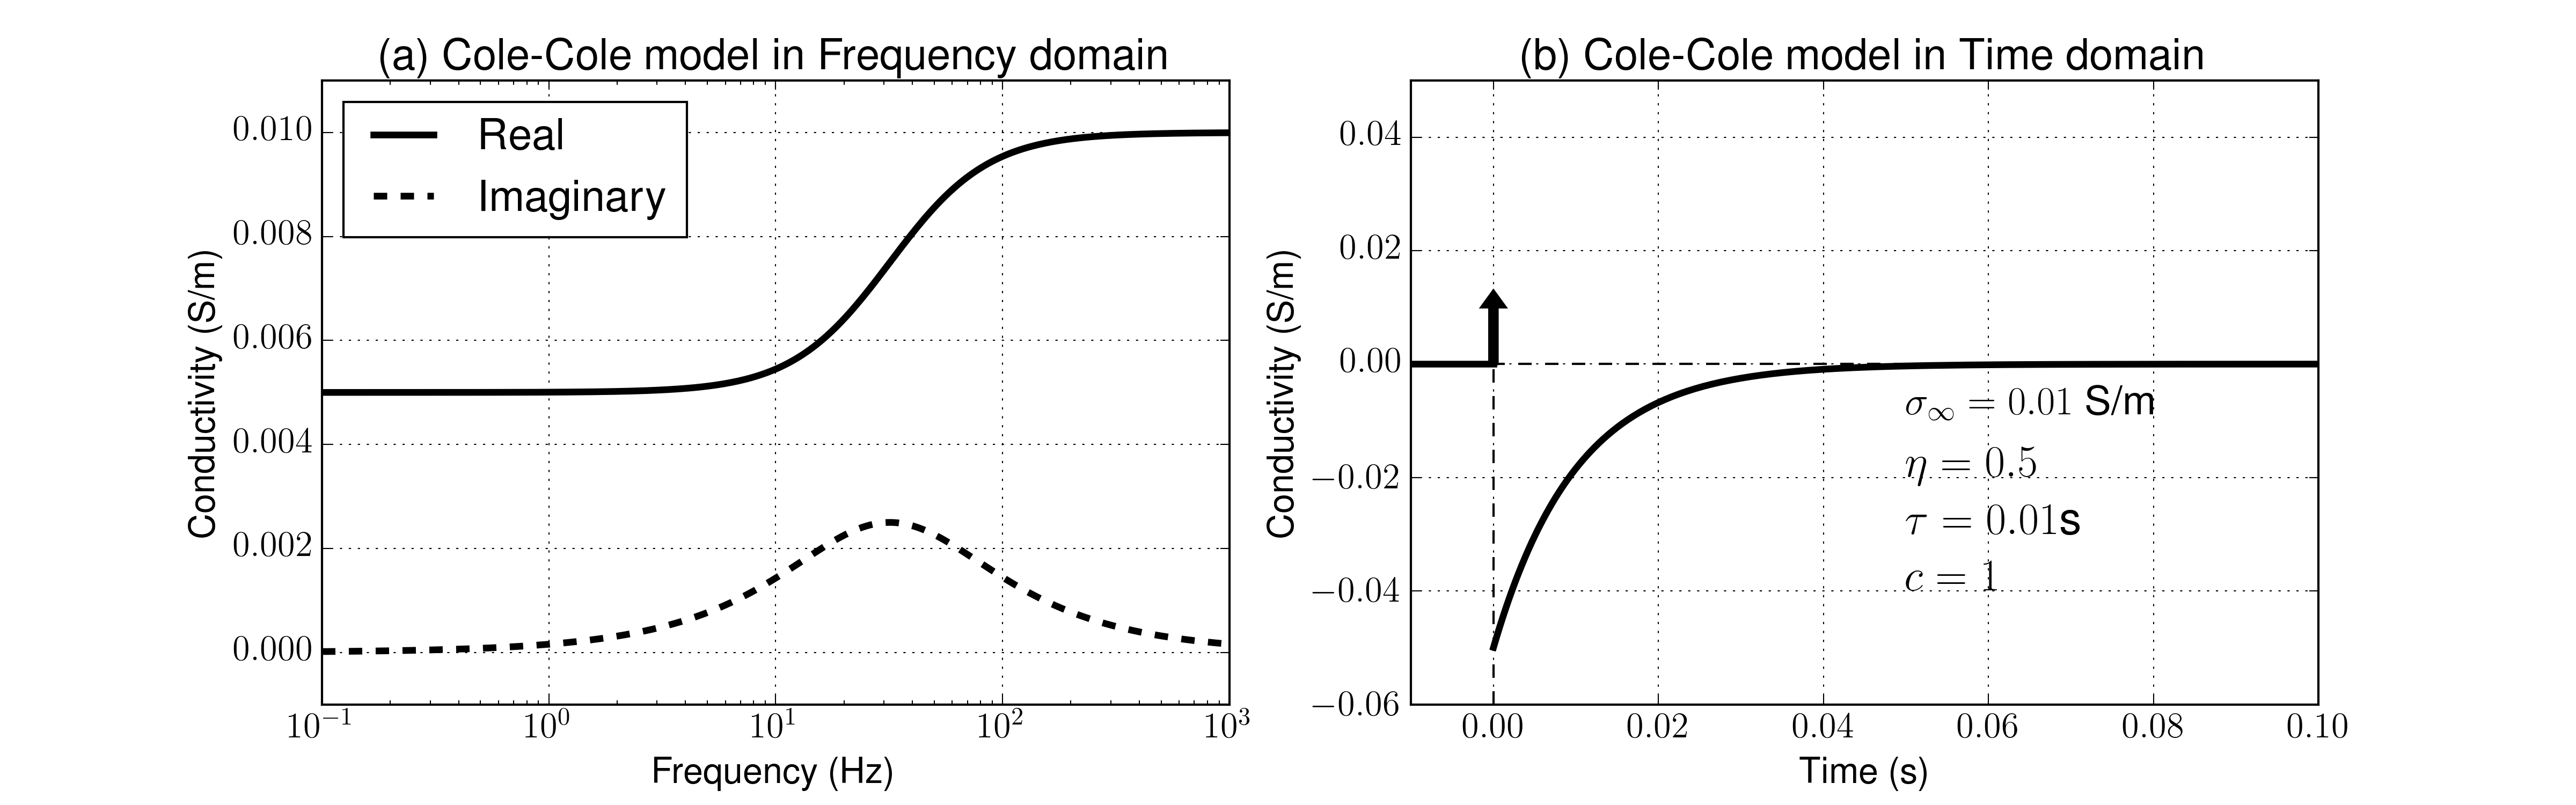
\includegraphics[width=1.0\textwidth]{figures/FDandTDCole.png}}
  \caption{Cole-Cole model in frequency domain (a) and time (b) domain. The Cole-Cole parameters are $\siginf$ = $10^{-2}$ S/m, $\eta $ = 0.5, $\tau$ = 0.01, and $c$=1.}
  \label{Fig:FDandTDCole}
\end{figure}

%% =============================================================================
%% Section. Decomposition of observed responses
%% =============================================================================

\section{Decomposition of observed responses}
IP effects in the observed data are coupled with EM effects. We need to decompose the observations to isolate data associated only with the IP phenomena.  
Maxwell's equations in the time domain, with a quasi-static approximation, are written as:
\begin{linenomath*}
\begin{equation}
  \curl{\e} = -\frac{\partial \b}{\partial t},
  \label{eq: total_farad}
\end{equation}
\end{linenomath*}
\begin{linenomath*}
\begin{equation}
  \curl{\frac{1}{\mu}\b} - \j= \j_{s},
  \label{eq: total_coulomb}
\end{equation}
\end{linenomath*}
where $\e$ is the electric field ($V/m$), $\b$ is the magnetic flux density ($Wb/m^2$) and $\mu$ is the magnetic permeability ($H/m$). Here $\j$ is the conduction current. In the frequency domain, this conduction current, $\J$ is related to conductivity via Ohm’s law: $\J(\omega) = \sigma(\omega)\E(\omega)$ where $\E$ is the electric field. 
Converting this relationship to time domain using the inverse Fourier transform yields:
\begin{linenomath*}
\begin{equation}
  \j(t) = \sigma(t)\otimes \e(t) = \int_0^t \sigma(u) e(t-u) du.
  \label{eq: ohms_law_convolution}
\end{equation}
\end{linenomath*}
where $\otimes$ indicates time convolution for a causal signal.  
Thus the current density depends upon the previous history of the electric field.
As in \cite{Smith1988a}, we represent total fields as $\e = \e^{F} + \e^{IP}$, $\b = \b^{F} + \b^{IP}$ and $\j = \j^{F} + \j^{IP}$, where superscript $F$ indicates fundamental and $IP$ is induced polarization. 
Here fundamental fields indicate EM fields without IP effects. 
Substituting into equations (\ref{eq: total_farad}) and (\ref{eq: total_coulomb}) yields the following sequences:
\begin{linenomath*}
\begin{equation}
  \curl({\e^{F}+\e^{IP}}) = -\frac{\partial}{\partial t} (\b^{F}+\b^{IP}),
\end{equation}
\end{linenomath*}
\begin{linenomath*}
\begin{equation}
  \curl\frac{1}{\mu}(\b^{F}+\b^{IP}) - (\j^{F}+\j^{IP})= \j_{s}.
\end{equation}
\end{linenomath*}

The fundmental equations can be written as
\begin{linenomath*}
\begin{equation}
  \curl \e^{F} = -\frac{\partial \b^{F}}{\partial t},
  \label{eq: eq_primary_farad}
\end{equation}
\end{linenomath*}
\begin{linenomath*}
\begin{equation}
  \curl{\frac{1}{\mu}\b^{F}} -\j^{F} = \j_s.
  \label{eq: eq_primary_coulomb}
\end{equation}
\end{linenomath*}
Here
\begin{linenomath*}
\begin{equation}
  \j^{F} = \siginf\e^{F}.
  \label{eq: jF}
\end{equation}
\end{linenomath*}

Substituting the fundamental fields into equations (\ref{eq: total_farad}) and (\ref{eq: total_coulomb}) yields the expressions for the IP fields 
\begin{linenomath*}
\begin{equation}
  \curl \e^{IP} = -\frac{\partial \b^{IP}}{\partial t},
  \label{eq: eq_secondary_farad}
\end{equation}
\end{linenomath*}
\begin{linenomath*}
\begin{equation}
  \curl{\frac{1}{\mu}\b^{IP}} = \j^{IP}.
  \label{eq: eq_secondary_coulomb}
\end{equation}
\end{linenomath*}

Let $F[\cdot]$ denote operator associated with Maxwell’s equations, and let $d$ denote the observations that include both EM and IP effects. 
Keeping the same notation, we can obtain $d = d^{F} + \dip$, where $d^F$ and $\dip$ are fundamental and IP responses, respectively. 
Based on this, we define the IP datum as 
\begin{linenomath*}
\begin{equation}
  \dip = d - d^{F} = F[\sigma(t)]-F[\siginf].
    \label{eq: IPdatum_syn}
\end{equation}
\end{linenomath*}
Here $F[\siginf]$ corresponds to the fundamental response ($d^F$). 
This subtraction process acts as an EM decoupling process, which removes the EM effects from the measured responses. This is the same procedure that formed the basis of work by \cite{routh2001}. 

%% ============================================================
%% Section. Pseudo-chargeability for inductive sources
%% ============================================================
\section{Pseudo-chargeability for inductive sources}
%% later
% A major difference of the inductive source from the galvanic source is the absence of the steady-state electric field. 
% This generates a principal difference on the IP response for both inductive and galvanic sources. 
% To examine this, we define the IP current ($\j^{IP}$) as
Combining equations (\ref{eq: sigma_time}) and  (\ref{eq: ohms_law_convolution}) writing $j(t)=j^F + j^{IP}$ we obtain
\begin{linenomath*}
\begin{equation}
  \j^{IP} = \siginf \e^{IP} + \j^{pol},
  \label{eq:IP_current}
\end{equation}
\end{linenomath*}
where the polarization current ($\j^{pol}$) is
\begin{linenomath*}
\begin{equation}
  \j^{pol}(t) = \dsig(t) \otimes \e(t).
  \label{eq:polarization_current}
\end{equation}
\end{linenomath*}

If the electric field has different characteristics for the inductive and galvanic sources this will generate different features in the polarization current.  
We consider two cases: a) galvanic source without EM induction and b) inductive source with EM induction. The first case corresponds to EIP \cite[]{seigel1959}, and the second is ISIP.
Figure \ref{F:DCEM_F_current} shows the amplitude of the fundamental electric field ($\e^{F}$) in the earth for those two cases. 
For the galvanic source, the electric field is instantaneous due to the steady-state electric field (Figure \ref{F:DCEM_F_current} (a)). 
However, for the inductive source, the electric field in the off-time is not zero, but increases to a peak and then decays as shown in Figure \ref{F:DCEM_F_current} (b). 
The polarization current for the two different sources will be significantly affected by these different electric fields. 
To capture this difference in a linearized kernel for the IP response, we define pseudo-chargeability ($\peta(t)$) as 
\begin{linenomath*}
\begin{equation}
  \peta(t) = -\frac{\j^{pol}(t)}{\j^{\ ref}},
  \label{eq:pseudochargeability_0}
\end{equation}
\end{linenomath*}
where the reference current ($\j^{ref}$) is defined as 
\begin{linenomath*}
\begin{equation}
  \j^{\ ref} = \siginf \eref.
  \label{eq:reference_current}
\end{equation}
\end{linenomath*}
Here $\eref$ is the reference electric field and both $\j^{\ ref}$ and $\eref$ are static fields that are independent of time. 
The pseudo-chargeability defined in equation (\ref{eq:pseudochargeability_0})  is the ratio of  the polarization current to the reference current. This is a small quantity and it plays an essential role in our linearization. 

To evaluate the pseudo-chargeability, we have to identify the reference current or reference electric fields. For the EIP case, the electric field, when there is no IP present, is independent of time as shown in Figure \ref{F:DCEM_F_current}(a). For the inductive source however, the electric field does not achieve a steady-state, but increases to a  peak then decreases. 

% Doug: May be later
% Moreover, the time history of the electric field will be different at each point in the earth. Our choice of the reference field is the value of $\e^{F}(t)$ at  the  time ($t^{\ ref}$) at which the  amplitude of the the electric field achieves its maximum value. 

Each pixel in the Earth has its own reference electric field and time thus  both $\eref$ and $t^{\ ref}$ have a 3D distribution. 
For both EIP and ISIP cases, we mathematically present our choice of the reference electric field as
\begin{linenomath*}
\begin{equation}
  \eref = \e^{F}(t) \otimes \delta(t-t^{\ ref}). 
  \label{eq:reference_electricfield}
\end{equation}
\end{linenomath*}
The reference time for the EIP case can be any time in the on-time, because the fundamental electric field for the EIP case does not change in on-time. 

By rearranging equation (\ref{eq:pseudochargeability_0}), we obtain 
\begin{linenomath*}
\begin{equation}
  \j^{pol} = -\jref\peta(t). 
  \label{eq:polarization_current_concept}
\end{equation}
\end{linenomath*}
This states that the polarization current has an opposite direction to the reference current, and is proportional to the pseudo-chargeability ($\peta(t)$). 
This conceptual model about the polarization current shown in equation (\ref{eq:polarization_current_concept}) is consistent with \cite{seigel1959}'s result. We note, that for any pixel, even though  $\eref$  attains the same value for an ISIP survey as for an EIP survey, the pseudo-chargeability resulting from  an ISIP survey  will be less than that from an EIP survey. We can infer from this that  linearization techniques, which  have worked so well in EIP problems, should be successful in ISIP problems. 

\begin{figure}  
  \figbox*{}{}{
  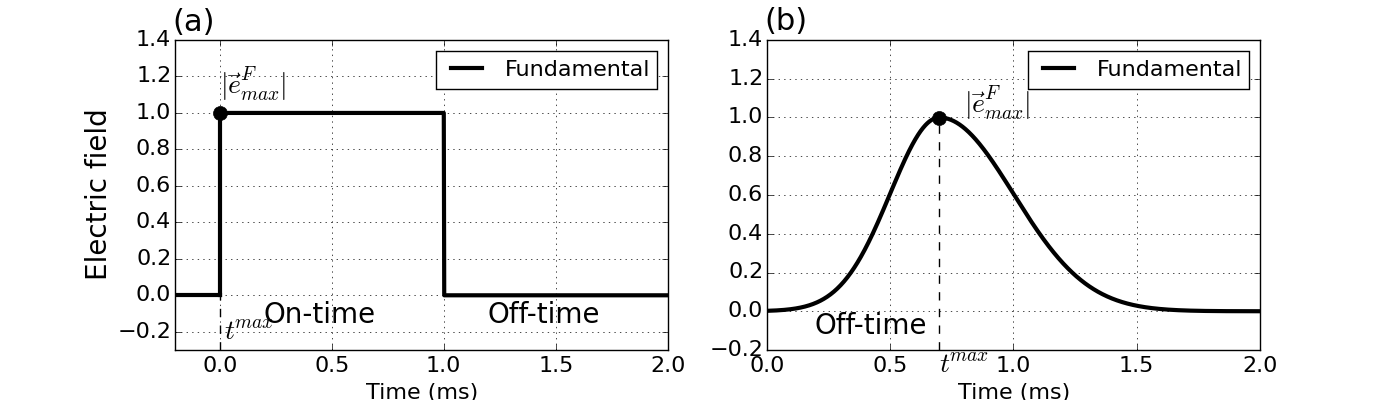
\includegraphics[width=1.0\textwidth]{figures/DCEM_F_current.png} }
  \caption{Conceptual diagram for the amplitude of the fundamental electric fields. (a) EIP and (b) ISIP cases.}
  \label{F:DCEM_F_current}
\end{figure}   

%% ============================================================
%% Section. Linearization
%% ============================================================
\section{Linearization}
Following from the methodologies in EIP, our goal is to express the IP response ($\dip$) as a function of the pseudo-chargeability $(\peta(t))$ in time  $\dip(t) = J[\peta(t)]$, where $J[\cdot]$ is a linear operator which is independent of time. In doing this we first consider a general EM system which is applicable to galvanic or inductive sources. 
For any pixel  volume in the earth the amplitude and direction of the  electric field can vary dramatically  in time and this results in a complicated  IP charging process. If substantial polarization currents are developed however, they will correspond to a maximum electric field or reference current aligned in a constant direction. Our formulation focuses on this aspect. We assume that the final large-scale IP response observed in the data is the result of  pixels being charged with an electric field in a specific direction but with a variable amplitude. Let $\e(t)$ be approximated as
\begin{linenomath*}
\begin{equation}
  \e(t) \approx \eref \hat{w}(t),
  \label{eq: e_with_eref}
\end{equation}
\end{linenomath*}
where $\hat{w}(t)$ is defined as:
\begin{linenomath*}
\begin{equation}
  \hat{w}(t) = P_0[w^{ref}(t)].
  \label{eq: we}
\end{equation}
\end{linenomath*}
Here a projection ($P_0[\cdot]$) of an arbitrary function, $f(t)$ is
\begin{linenomath*}
\begin{equation}
  P_0[f(t)] = \left\{ 
  \begin{array}{l l}
    f(t) & f(t) \ge 0 \\
    0 & \text{if } f(t) < 0, 
  \end{array}\right.
  \label{eq: P0}
\end{equation}
\end{linenomath*}
and
\begin{linenomath*}
\begin{equation}
  w^{ref}(t) = \frac{\e^F(t)\cdot\eref}{\eref\cdot\eref}.
  \label{eq: wref}
\end{equation}
\end{linenomath*}
Here $w^{ref}(t)$ is a dimensionless function that prescribes the time history of the electric field at each location along the direction of the chosen reference electric field ($\eref$).  Negative values of  $w^{ref}(t)$ are set to zero in accordance with our conceptual model that polarization currents have an opposite direction to the reference current (equation (\ref{eq:polarization_current_concept})).
We redefine the pseudo-chargeability as
\begin{linenomath*}
\begin{equation}
    \peta(t) = \peta^{I}(t)\otimes \hat{w}(t).
    \label{eq: pseudochargeability}
\end{equation}
\end{linenomath*}
The polarization current, $\j^{pol}$ can be approximated with equation (\ref{eq: intrinsic_peta}) as
\begin{linenomath*}
\begin{equation}
  \j^{pol}(t) \approx - \peta^{I}(t)\otimes \hat{w}(t)\jref.
\end{equation}
\end{linenomath*}
Substituting this into equation (\ref{eq:IP_current}) yields
\begin{linenomath*}
\begin{equation}
  \j^{IP}(t) \approx \siginf\e^{IP}(t) - \peta^{I}(t)\otimes \hat{w}(t)\jref
\end{equation}
\end{linenomath*}
and this yields
\begin{linenomath*}
\begin{equation}
  \j^{IP}(t) \approx \siginf\e^{IP}(t) -\jref\peta(t).
  \label{eq: jip_EMIP}
\end{equation}
\end{linenomath*}

The second term, $-\jref\peta(t)$, correspond to polarization currents. The first term, $\siginf e^{IP}(t)$ is usually omitted \cite[]{Smith1988a}. Here we include it and explore the conditions in which it is important. 
Because the reference current is static, any time-dependency in the polarization currents is encapsulated in the pseudo-chargeability. The buildup and decrease of polarization currents is a slow process and we assume therefore that this process does not produce induction effects ($\frac{\partial \b^{IP}}{\partial t} \approx 0$) and therefore we can write 
\begin{linenomath*}
\begin{equation}
  \e^{IP} \approx  \e^{IP}_{approx} = -\grad\phi^{IP}.
  \label{eq: eip_approx}
\end{equation}
\end{linenomath*}

By taking the divergence of  equation (\ref{eq: jip_EMIP}), substituting  $\e^{IP}$ with equation (\ref{eq: eip_approx}), and carrying out some linear algebra, we obtain
\begin{linenomath*}
\begin{equation}
  \phi^{IP}(t) \approx -[\div \siginf\grad]^{-1}\div\jref\peta(t).
  \label{eq: phiIPapprox_general}
\end{equation}
\end{linenomath*}
By applying the gradient we obtain 
\begin{linenomath*}
\begin{equation}
    \e^{IP}_{approx} = \grad[\div \siginf\grad]^{-1}\div\jref\peta(t).
    \label{eq: eip_approx_full}
\end{equation}
\end{linenomath*}
Thus, the electric field due to the IP effect can be expressed as a function of $\peta(t)$ in time. 
This form is also applicable to the  EIP case.   

For an inductive source, the data is often either $\b$ or its time derivative and hence we also need to compute $\b^{IP}$ or its time derivative.
For this, we first compute $\j^{IP}$ then use the Biot-Savart law. 
By substituting equation (\ref{eq: eip_approx_full}) into equation (\ref{eq: jip_EMIP}), the approximated IP current density, $\j^{IP}_{approx}$ can be expressed as
\begin{linenomath*}
\begin{equation}
  \j^{IP}(t) \approx \j^{IP}_{approx} = \bar{S}\jref\peta(t),
  \label{eq: jip_approx}
\end{equation}
\end{linenomath*}
where
\begin{linenomath*}
\begin{equation}
  \bar{S} = \siginf\grad[\div \siginf\grad]^{-1}\div-\bar{I}
\end{equation}
\end{linenomath*}
and $\bar{I}$ is an identity tensor. 
Applying the Biot-Savart law we have:
\begin{linenomath*}
\begin{equation}
  \b^{IP}_{approx}(\vec{r}; t) = \frac{\mu_0}{4\pi}\int_{\Omega}  \frac{\bar{S}\j^{\ ref}(\vec{r}_s)\times\hat{r}}{|\vec{r}-\vec{r}_s|^2}\peta(t)d\vec{r}_s.
  \label{eq: BiotbIP_approx}
\end{equation}
\end{linenomath*}
If $\siginf\e^{IP}$ is omitted in  $\j^{IP}$ then the tensor, $\bar{S}$ becomes $-\bar{I}$. 
In this situation, the IP current is same as the polarization current, and it always has opposite direction to the reference current. 
This reversed current, along with Biot-Savart law,  provides a physical understanding about the negative transients in ATEM data when the earth is chargeable. 

Observed data are often the time derivative of $\b$, hence by taking time derivative to the equation (\ref{eq: BiotbIP_approx}), we obtain
\begin{linenomath*}
\begin{equation}
  -\frac{\partial\b^{IP}_{approx}}{\partial t}(\vec{r}; t) = \frac{\mu_0}{4\pi} \int_{\Omega}  \frac{\bar{S}\jref(\vec{r}_s)\times\hat{r}}{|\vec{r}-\vec{r}_s|^2} \Big( -\frac{\partial \peta(t)}{\partial t} \Big) d\vec{r}_s.
  \label{eq: BiotbIPdt_approx}
\end{equation}
\end{linenomath*}
Here we have chosen to keep the minus signs in equation (\ref{eq: BiotbIPdt_approx}) so that $-\frac{\partial \peta(t)}{\partial t}$ is positive when $\peta(t)$ is decaying in time. 
Accordingly, the IP datum is given by  $-\frac{\partial\b^{IP}}{\partial t}$. 

The IP fields shown in equations (\ref{eq: eip_approx_full}), (\ref{eq: BiotbIP_approx}) and (\ref{eq: BiotbIPdt_approx}) are linear functionals of $\peta$ and the equations for a single time channel can be discretized in space as
\begin{linenomath*}
\begin{equation}
  \mathbf{d}^{IP} = \mathbf{J}\peta,
  \label{eq: dIP_lineareq}
\end{equation}
\end{linenomath*}
where $\mathbf{J}$ is the corresponding sensitivity matrix. 
In particular when the observed datum is the time derivative of $\b$, the linear relationship can be written as 
\begin{linenomath*}
\begin{equation}
  \mathbf{d}^{IP} = \mathbf{J}(-\frac{\partial \peta}{\partial t}\Big|).
  \label{eq: dIP_lineareq_dbdt}
\end{equation}
\end{linenomath*}
A detailed description for the discretization of the linearized kernel is shown in Appendices \ref{section:maxwell_discrete} and \ref{section:linearkernel_discrete}. 
The representation in equation (\ref{eq: dIP_lineareq}) is valid for galvanic and inductive sources but the two assumptions: a) $\e \approx \eref \hat{w}(t)$ and b) $\e^{IP} \approx -\grad\phi^{IP}$ need to be tested numerically for the case of inductive sources. 

%% =============================================================================
%% Section. IP inversion methodology
%% =============================================================================

\section{IP inversion methodology}

%%% ===========================================================================
%%% SUBSECTION
\subsection{3D IP inversion with a linearized kernel}
The linear inverse problem to recover chargeability is straightforward and is described in \cite{doug1994}. 
We rewrite equation (\ref{eq: dIP_lineareq}) as
\begin{linenomath*}
\begin{equation}
  \mathbf{d}^{pred} = \mathbf{J}\mathbf{m},
  \label{eq9}
\end{equation}
\end{linenomath*}
where $\mathbf{J}$ is the  sensitivity matrix of linear problem, which corresponds to $\mathbf{J}$ shown in equation (\ref{eq: dIP_lineareq}) 
Here, $\mathbf{d}^{pred}$ represents IP responses at a single time channel, $\mathbf{m}$ disturbs model parameters, which can be either $\peta$ or $-\frac{\partial \peta}{\partial t}\big|$ at the same time. 
In our work here we invert each time channel of $d^{IP}$, separately. 

The solution to the inverse problem is the model $\mathbf{m}$ that solves the optimization problem
\begin{linenomath*}
\begin{equation}
  minimize \ \phi =  \phi_d(\mathbf{m}) + \beta\phi_m(\mathbf{m}) \\
  s.t. \ 0 \le \mathbf{m},
  \label{eq10}
\end{equation}
\end{linenomath*}
where $\phi_d$ is a measure of data misfit, $\phi_m$ is a user-defined model objective function and $\beta$ is regularization or trade-off parameter. We solve this optimization problem using a projected Gauss-Newton method \cite[]{Kelley}. 
The value of $\beta$ in the iteration of this non-linear inversion is determined using a cooling technique where $\beta$ is progressively reduced from some high value. The inversion is stopped when the tolerance is reached (cf. \cite{DougTutorial, Kang2014}). 

We use the sum of the squares to measure data misfit
\begin{linenomath*}
\begin{equation}
  \phi_d = \| \mathbf{W_d}(\mathbf{A}\mathbf{m}-d^{obs}|)\|^2_2 =
  \sum^N_{j=1}(\frac{\mathbf{d}^{pred}_j-\mathbf{d}^{obs}_j}{\epsilon_j}),
  \label{eq11}
\end{equation}
\end{linenomath*}
where $N$ is the number of the observed data and $\mathbf{W_d}$ is a diagonal data weighting matrix which contains the reciprocal of the estimated uncertainty of each datum ($\epsilon_j$) on the main diagonal,  $\mathbf{d}^{obs}$ is a vector containing the observed data, $\mathbf{d}^{pred}$ is a vector containing calculated data from a linear equation given in equation (\ref{eq9}).
The model objective function, $\phi_m$, is a measure of the amount structure in the model and upon minimization this will generate a smooth model which is close to a reference model, $m_{ref}$. 
We define $\phi_m$ as
\begin{linenomath*}
\begin{equation}
  \phi_m = \sum_{i=s,x,y,z} \alpha_i\| \mathbf{W}_i\mathbf{W}(\mathbf{m}-\mathbf{m}_{ref})\|^2_2,
  \label{eq12}
\end{equation}
\end{linenomath*}
where $\mathbf{W}_s$ is a diagonal matrix, and $\mathbf{W}_x$, $\mathbf{W}_y$ and $\mathbf{W}_z$ are discrete approximations of the first derivative operator in $x$, $y$ and $z$ directions, respectively.  
The $\alpha$'s are weighting parameters that balance the relative importance of producing small or smooth models.

Because we are inverting each time channel of $\dip$ datum, separately, we may not have intrinsic depth resolution. This could be overcome if there were multiple receivers for each transmitter, although usual ATEM surveys only have a single receiver. To compensate for this, and similar to the magnetic inversion \cite[]{LiMag3D}, we apply a depth weighting through model weighting matrix ($\mathbf{W}$):
\begin{linenomath*}
\begin{equation}
    \mathbf{W} = \mathbf{diag}(\mathbf{z-z_0})^{1.5},
    \label{eq: weight_mat}
\end{equation}
\end{linenomath*}
where $\mathbf{z}$ and $\mathbf{z_0}$ are discretized depth locations and reference depth in the 3D domain.
For the implementation of our IP inversion algorithm, we use an open source python package for simulation and gradient-based parameter estimation in geophysics called SimPEG \cite[]{Cockett2015}. 

%% ===========================================================================
%% SUBSECTION
\subsection{Extracting intrinsic IP parameters}
\label{section: extract_intrinsicIP}
The output of our IP inversion is a 3D distribution of the pseudo-chargeability at multiple time channels. 
As its name suggests, pseudo-chargeability is not an intrinsic IP parameter like chargeability, but it is a convoluted property between $\peta^{I}(t)$ and $\hat{w}(t)$:
\begin{linenomath*}
\begin{equation}
  \peta(t) = \peta^{I}(t) \otimes \hat{w}(t),
  \label{eq: pseudochargeability_petaI}
\end{equation}
\end{linenomath*}
with the definition of intrinsic pseudo-chargeability (equation (\ref{eq: intrinsic_peta})).
We would now like to use the $\peta(t)$ as the “data” and recover intrinsic parameters such as $\eta, \tau, c$ in a Cole-Cole model. Assuming a Debye model ($c$=1), we obtain
\begin{linenomath*}
\begin{equation}
    \peta^{I}(t) = \frac{\eta}{(1-\eta)\tau}e^{-\frac{t}{(1-\eta)\tau}},
    \label{eq: intrinsic_peta_debye}
\end{equation}
\end{linenomath*}
Since we have $\siginf$ we can compute $\hat{w}(t)$, which is the time history of the electric field. 
Accordingly, we can unravel the recovered pseudo-chargeability to extract intrinsic IP parameters such as chargeability($\eta$) and time constant ($\tau$). 
We use a gradient-based optimization and thus we need the sensitivity function for the pseudo-chargeability (equation (\ref{eq: pseudochargeability_petaI})) with respect to $\eta$ and $\tau$. 
To simplify this procedure, we rewrite intrinsic pseudo-chargeability as 
\begin{linenomath*}
\begin{equation}
  \peta^{I}(t) = a e^{-bt},
\end{equation}
\end{linenomath*}
where $a = \frac{\eta}{(1-\eta)\tau}$ and $b = \frac{1}{(1-\eta)\tau}$. 
Then we take derivative of $\peta(t)$ with regard to $a$ and $b$:
\begin{linenomath*}
\begin{equation}
  \frac{\partial \peta(t)}{\partial a} = e^{-bt} \otimes \hat{w}(t),
\end{equation}
\end{linenomath*}
\begin{linenomath*}
\begin{equation}
  \frac{\partial \peta(t)}{\partial b} = -ate^{-bt} \otimes \hat{w}(t).
\end{equation}
\end{linenomath*}
With these sensitivity functions, we can set up an inverse problem, and recover $a$ and $b$. 
Chargeability and time constant can be obtained by using $a$ and $b$:
\begin{linenomath*}
\begin{equation}
  \eta =  \frac{a}{b},
\end{equation}
\end{linenomath*}
\begin{linenomath*}
\begin{equation}
  \tau =  \frac{1}{(1-a/b)b}.
\end{equation}
\end{linenomath*}
We apply this inversion separately to each cell in the recovered pseudo-chargeability  in a manner similar to \cite[]{Yuval1997}.
For the better representation of time-dependent conductivity, a different parameterization such as stretched-exponential \cite[]{Kohlrausch1854} or Cole-Cole model with variable $c$ can be implemented. 

% %%% ===========================================================================
% %%% SUBSECTION
\subsection{Handling multiple transmitters in ATEM surveys}
\label{subsection: Handling multiple transmitters in ATEM surveys}
The work for inductive sources in the previous sections has been developed for a single transmitter and 3D information about chargeability can be obtained if there are multiple receivers. For ATEM data however, we have only a single receiver location for each transmitter but we have multiple transmitter locations. 
Our goal is to alter the problem to work with an effective pseudo-chargeability. 

In our linearized equation (\ref{eq9}), each transmitter has its own sensitivity and pseudo-chargeabilty. For our airborne case the sensitivity for the $k$-th transmitter is the $k$-th row of $\mathbf{J}$ and the pseudo-chargeability is $\peta^k$. The corresponding  IP datum is 
\begin{linenomath*}
\begin{equation}
  \dip_k(t) = \sum_{i=1}^{nC}J_{k,i}\peta^k_i (t), \ \ k=1, \ldots, nTx,
  \label{eq: dip_kthTx}
\end{equation}
\end{linenomath*}
where $nTx$ is the number of transmitters, $nC$ is the number of cells in the domain, and $J_{k,i}$ indicates an element of the Jacobian matrix for the $k$-th transmitter and the $i$-th cell. We want to replace $\peta^k_i$ with a single effective pseudo-chargeabilty $\peta^k$ and therefore write the IP datum as 
\begin{linenomath*}
\begin{equation}
  \dip_k(t) = \sum_{i=1}^{nC}J_{k,i}\peta_i (t), \ \ k=1, \ldots, nTx,
  \label{eq: dipeff_kthTx}
\end{equation}
\end{linenomath*}
The waveforms are different for each transmitter and hence this representation cannot be exact. To examine the implications of this it suffices to look at the contribution of any volumetric pixel. Each pixel contributes to all of the IP data but in differing amounts. The total contribution of the  $i$-th pixel to the $nTx$ data set at a single time is  
\begin{linenomath*}
\begin{equation}
  q_i =\sum_{k=1}^{nTx} J_{k,i} \peta^k_i(t), \ \ i=1, \ldots, nC.
  \label{eq: dip_hat}
\end{equation}
\end{linenomath*}
Our goal is to find an effective chargeability that produces the same net effect on the measured data. We search for a transmitter-independent $\peta_i$ such that 
\begin{linenomath*}
\begin{equation}
  q_i^{est} =\sum_{k=1}^{nTx} J_{k,i} \peta_i(t), \ \ i=1, \ldots, nC.
  \label{eq: dip_tilde}
\end{equation}
\end{linenomath*}
Minimizing the least squares difference between equations (\ref{eq: dip_hat}) and (\ref{eq: dip_tilde}) yields
\begin{linenomath*}
\begin{equation}
  \peta_i(t) = \frac {\Sigma_{k=1}^{nTx} J_{k,i}^2\peta^k_i(t)} {\Sigma_{k=1}^{nTx} J_{k,i}^2} = \sum_{k=1}^{nTx} a^k_i \peta^k_i(t), \ \ i=1, \ldots, nC.
  \label{eq: petaeff}
\end{equation}
\end{linenomath*}
where normalized weight ($a^k_i$) is 
\begin{linenomath*}
\begin{equation}
  a^k_i = \frac {J^2_{k,i}} {\Sigma_{k=1}^{nTx} J^2_{k,i}}, \ \ i=1, \ldots, nC.
  \label{eq: normalized_weights}
\end{equation}
\end{linenomath*}

With the above understanding about how $\peta_i$ relates to the $\peta_i^k$ from each transmitter we can proceed  as follows. Firstly, from equation (\ref{eq: pseudochargeability}) we have 
\begin{linenomath*}
\begin{equation}
  \peta_i^k(t) =\peta^I \otimes \hat{w}^{k}_i(t) 
  \label{eq: peta_transmitters}
\end{equation}
\end{linenomath*}
Substituting \ref{eq: peta_transmitters} into \ref{eq: petaeff} allows us to write
\begin{linenomath*}
\begin{equation}
  \peta_i(t) = \peta^I(t) \otimes w^e_i(t),
\end{equation}
\end{linenomath*}
where we define effective time history of the electric field, $w^e_i(t)$ as 
\begin{linenomath*}
\begin{equation}
  w^e_i(t)= \sum_{k=1}^{nTx} a^k_i \hat{w}^{k}_i(t), \ \ i=1, \ldots, nC.
  \label{eq: we_eff}
\end{equation}
\end{linenomath*}

The above equations shows that the pseudo-chargeabilty for any pixel recovered from the inversion is equal to the convolution of the intrinsic pseudo-chargeability ($\peta^I(t)$) with an effective time history of the electric field ($w^e(t)$). Although it is somewhat involved, the $w^e(t)$ associated with each pixel can be evaluated by knowing the electric fields associated with the fundamental EM problem. Ultimately this allows us to estimate the parameters associated with the intrinsic pseudo-chargeability in the same manner as outlined for the case with a single transmitter. Our ability to evaluate the $w^e(t)$ and test the validity of equation (\ref{eq: dipeff_kthTx}) will be treated in Section \ref{subsection: Effective pseudo-chargeability for ATEM data}.  

% Doug
% This includes all grounded surveys with multiple transmitters and to a single source inductive EIP surveys.

%%% ===========================================================================
%%% SUBSECTION
\subsection{IP inversion procedure}
As seen in the previous sections the extraction of IP information from TEM data has multiple steps. These include: (1) invert TEM data and recover a 3D conductivity model ($\sigma_{est}$). 
(2) Forward model $\sigma_{est}$ to obtain the fundamental response $d^F$ and subtract it from the observations to obtain $\dip$ data.
(3) Invert  $\dip$ data to recover pseudo-chargeability model at individual time channels using the relationship in equation (\ref{eq: dIP_lineareq}). 
(4) Further, process the inversion outputs at multiple time-channels  to estimate the Cole-Cole, or equivalent IP parameters.

In the following we investigate each of the above steps via numerical simulations and test the validity of our assumptions. 

%% =============================================================================
%% Section. Numerical experiments
%% =============================================================================

\section{Numerical experiments}
\label{section: numerical_examples}
For our numerical experiments we concentrate upon coincident loop ATEM surveys. This choice is made because of the observed negative transients that are direct indicators of IP phenomena \cite[]{Kratzer2012,Kang2015a,Kang2015b}, and the extensive  use of this survey  by industry.  

We begin with a simple IP model composed of  a chargeable block in a half-space as shown in Figure~\ref{F: IPModel}.
Cole-Cole parameters of  the block are  $\eta=$0.2, $\tau=$0.005 and $c=$1.
The conductivity  of the half-space, ($\sigma_1$) is  $10^{-3}$ S/m, whereas $\sigma_2$, 
the conductivity at infinite frequency, $\siginf$,  for the chargeable body, is variable.  
We consider three cases: a) canonical ($\sigma_2=\sigma_1$), b) conductive ($\sigma_2=10^2\times\sigma_1$) and c) resistive models ($\sigma_2=10^{-2}\times\sigma_1$).
The 3D earth is discretized with  $50\times50\times50$ m core cells and the number of cells in the domain is $41\times41\times40$.
The size of the chargeable body is $250\times250\times200$ m and the top boundary is located  $50$ m below the surface.
The EMTDIP code \cite[]{Marchant2014} is used to compute forward ATEM responses that include IP effects. The survey consisting of 11 soundings along each of 11 lines is shown in Figure \ref{F: IPModel}a.
Data are from a  coincident-loop system and both Tx and Rx are located 30 m above the surface; the radius of the loop is 10 m.
A step-off transmitter waveform is used and the range of the observed time channels is 0.01-60 ms. The observed responses can be the vertical component of $\b$ or $\frac{\partial \b}{\partial t}$.

In this section, we first decompose the observed responses and the total currents into fundamental and IP portions to aid in the basic understanding of IP effects in ATEM data. 
Second, we validate the linearized functional by computing the approximate IP current and IP responses, and compare these  with the true values. 
Third, we investigate the feasibility of detecting an effective pseudo-chargeability in 3D IP inversion when multi-transmitters are used. 
Fourth, we invert the IP data and recover 3D distributions of pseudo-chargeability at multiple times.  Lastly, we use the recovered pseudo-chargeabilities to examine the potential to extract intrinsic Cole-Cole parameters. 

\begin{figure}
  \figbox*{}{}{
  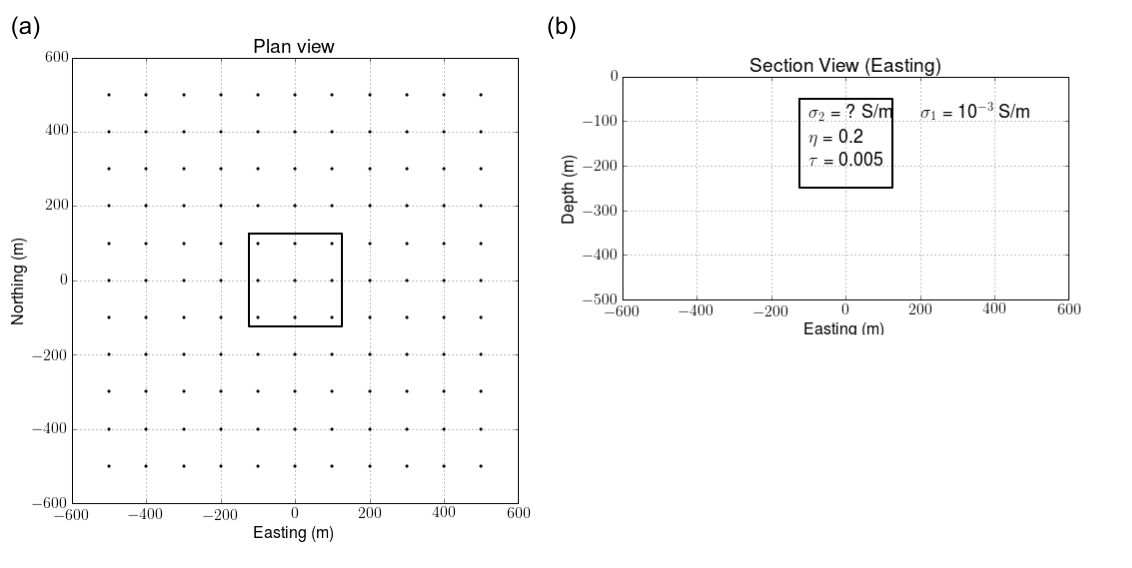
\includegraphics[width=1.0\textwidth]{figures/IPModel.png} }
  \caption{Plan (a) and section b) views of the IP model. The solid line in (a) delineates the boundary of the IP body. Solid circles in (a) denote the sounding locations. In (b) the conductivity $\sigma_2$ is variable so that  canonical, conductive and resistive blocks can be examined}
  \label{F: IPModel}
\end{figure}
\clearpage

%%% ===========================================================================
%%% SUBSECTION
\subsection{IP responses}
Using the  EMTDIP code and carrying out two simulations, we compute the IP data via subtraction in equation (\ref{eq: IPdatum_syn}).
Figure \ref{F:Three_IPresp} shows the observed, fundamental, and IP responses at a sounding location above the center of the chargeable body for (a) canonical, (b) conductive and (c) resistive models. Both $b_z$ and $-\frac{\partial b_z}{\partial t}$ data are shown. 
The IP effects are most noticeable for the conductive body and we turn attention to this example first. The IP response starts to significantly affect the observations near 0.6 ms and the observed responses show a sign reversal near 1 ms. Beyond that time the signal is dominated by the IP. The dashed line in Figure \ref{F:Three_IPresp}b shows that after turning off the transmitter current, the IP current increases (as inferred by the magnitude of the $b_z$ field) until about 1 ms and then decreases. We interpret this in terms of charging and discharging phases and a vertical dashed line in the figure defines the two phases. In the charging phase at early times the EM effects dominate and IP signals are not expected to be observed. In the discharging phase, which occurs at  later time, the IP effects may eventually dominate the EM effects. The maximum of the $b_z^{IP}$ corresponds to the zero crossing for $\frac{\partial b_z^{IP}}{\partial t}$ but the times at which the IP signal becomes dominant are delayed compared to $b_z^{IP}$. By comparing the observations with the fundamental fields we see that the IP signal could be recognized in the $b_z$ data near 0.7 ms and near 2.0 ms in the $\frac{\partial b_z}{\partial t}$ data.

The plots for the canonical and resistive bodies show that the time that separates charging and discharging occurs earlier than for the conductive body. This is a reflection that the fundamental currents reside for a longer time in a conductor. For the canonical body, a significant difference between the measured responses and the fundamental fields occur about 0.9 ms for $b_z$ and about 2 ms for $\frac{\partial b_z}{\partial t}$. The amplitudes of the IP responses are significantly smaller than those for the conductor.  Lastly, there is little IP signal for the resistive body; the IP signal is much smaller than the fundamental response throughout the given time range. This is a consequence of the small fundamental currents in the resistor. 

The decay curves from a sounding location  provide insight about the IP response but more is gleaned by looking at data from all  sounding locations in the ATEM survey. We focus on $b_z^{IP}$ for the conductive block at selected time channels. Figure \ref{F:IPresp_Plan} shows interpolated maps of the observed, fundamental and IP responses at (a) 0.86 ms and (b) 6.7 ms which are respectively included in the charging and discharging times. For the conductive block, 0.86 ms is close to the peak time when transition from charging to discharging occurs, but it is still included in the charging time. 
At this time, the observations are dominated by the fundamental response and no negative values,  which are the signature of the IP effect, are observed. Subtracting the fundamental however, yields a residual $\dip$ data map that has a strong negative. This  example  shows that our EM decoupling procedure can  work satisfactorily.  At 6.7 ms, obtaining good IP data are easier because the observed data already show negative values. There is still a weak fundamental field and the subtraction process improves the $\dip$ response. The $\dip$ data at  0.86 ms and 6.7 ms shown in Figure \ref{F:IPresp_Plan} are of sufficient quality to be inverted. 

\begin{figure}
  \figbox*{}{}{
  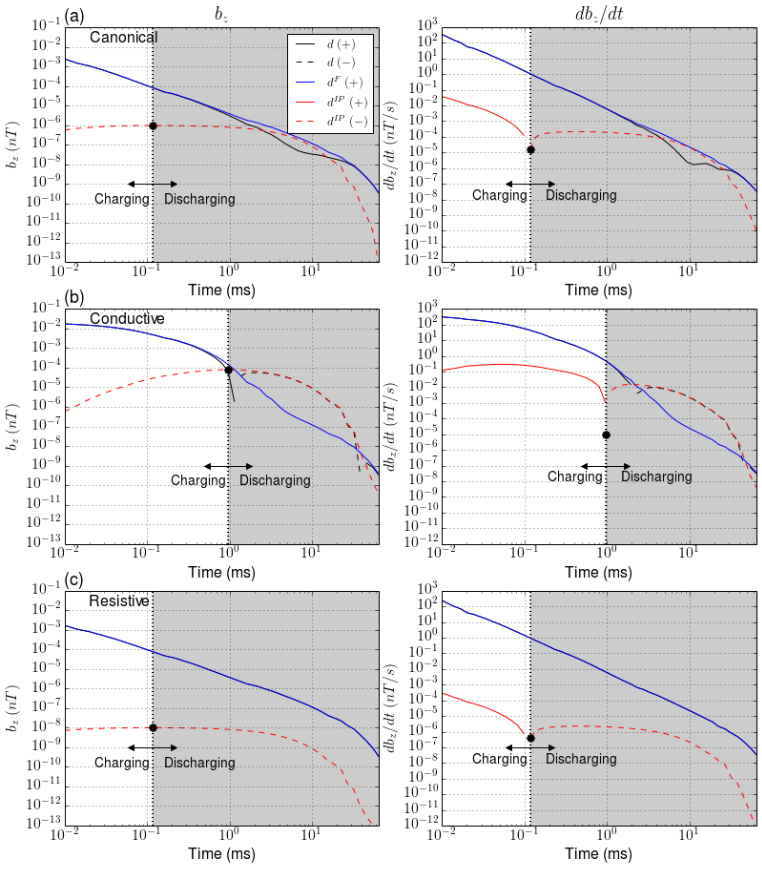
\includegraphics[width=1.\textwidth]{figures/Three_IPresp.png} }
  \caption{Time decaying curves of the observations  ($d$; black line), fundamental ($d^F$; blue line) and IP ($\dip$; red line) responses. All three cases: (a) canonical, (b) conductive and (c) resistive are presented. Right and left panels show $b_z$ and $\frac{\partial b_z}{\partial t}$. Black dotted line indicates the maximum polarization time.}
  \label{F:Three_IPresp}
\end{figure}
\begin{figure}
  \figbox*{}{}{
  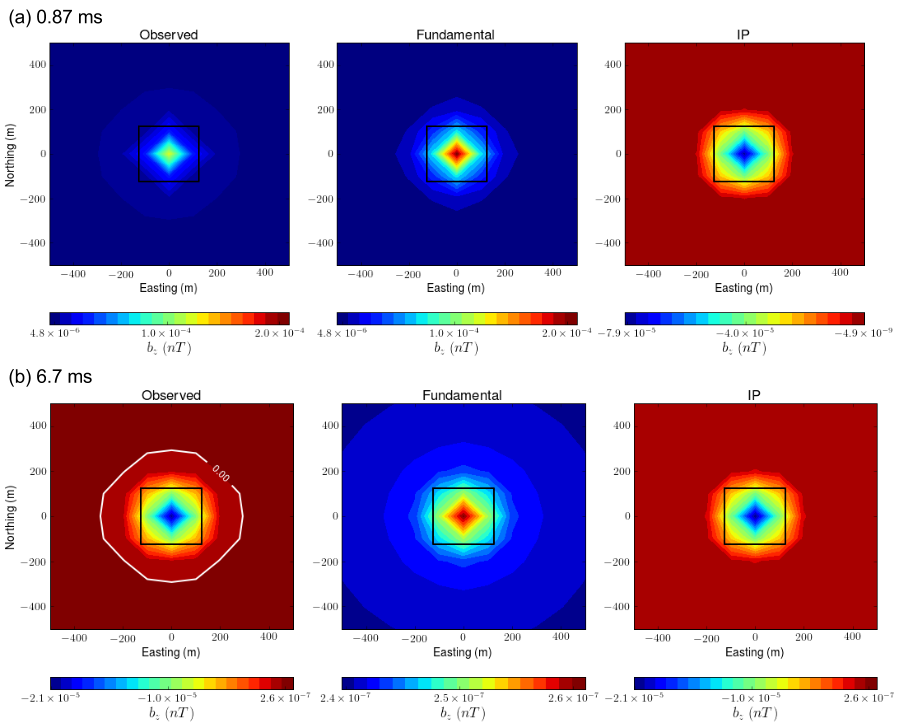
\includegraphics[width=1.\textwidth]{figures/IPresp_Plan.png} }
  \caption{Interpolated maps of observed (left panel), fundamental (middle panel) and IP (right panel) responses. Two time channels at (a) 0.86 ms and (b) 6.7 ms are presented. White line contours a zero-crossing in the observed response.  
  }
  \label{F:IPresp_Plan}
\end{figure}
\clearpage

%%% ===========================================================================
%%% SUBSECTION
\subsection{Polarization currents}
% Doug: What exactly is this section verifying wrt to any approximations?
To evaluate the polarization current shown in equation (\ref{eq:polarization_current}) for the linear functional, we assumed $\e(t) \approx \eref w^e(t)$ and defined our reference current as $\j^{ref}=\siginf \eref$. That yielded our approximation of the polarization current to be $\j^{pol}(t) \approx -\j^{\ ref} \peta(t)$. This approximation says that the polarization current has a fixed direction antiparallel to the reference current and that direction is the same for all times. The only time dependence occurs through the scalar $\peta(t)$. 

We investigate this by evaluating both reference and polarization currents numerically. 
From equation (\ref{eq:reference_electricfield}), a reference current can be considered as the maximum fundamental current that occurred throughout the  time history. 
To evaluate polarization currents we rearrange equation (\ref{eq:IP_current}) as $\j^{pol} = \j^{IP} - \siginf\e^{IP}$. Computation of this subtraction yields the polarization currents. 

Here we limit our attention to canonical and conductive blocks. 
Figures ~\ref{F:ReferenceCurrent}(a)   and (b) show reference currents for the canonical and conductive blocks, respectively. 
A transmitter is located at (-200 m, 0 m, 30 m) and marked as a white solid circle in the figure, where ($\cdot, \cdot, \cdot$) means a point at (easting, northing, depth).
Reference currents for the canonical block are circular, centered on the transmitter location, and decay with distance. 
For the conductive block, additional vortex currents are induced.
We compare these reference currents with the polarization currents. 
Figure ~\ref{F:Polarizationcurrent_early} shows the plan and section view maps of the polarization currents at 0.86 ms.
Comparisons of Figures ~\ref{F:ReferenceCurrent} and ~\ref{F:Polarizationcurrent_early} clearly show that polarization currents for both canonical and conductive blocks are oppositely aligned with respect to their reference current. This was the hypothesized outcome.
Figure ~\ref{F:Polarizationcurrent_late} show polarization currents at 6.7 ms, and direction of polarization currents are similar to those at 0.86 ms. 
This illustrates that direction of polarization currents after 0.86 ms for both canoncial and conductive blocks are almost constant in time. 

For an EIP survey conducted over one of the blocks, we expect  IP responses that could be explained by an electric dipole current in a chargeable medium \cite[]{seigel1959}. 
However, for the ISIP additional complexity arises due to vortex currents induced in a conductor because these generate complicated polarization currents within the chargeable medium. 
Our choice of reference currents effectively incorporates this complicated direction of polarization currents for a conductive medium. 

\begin{figure}
  \figbox*{}{}{
  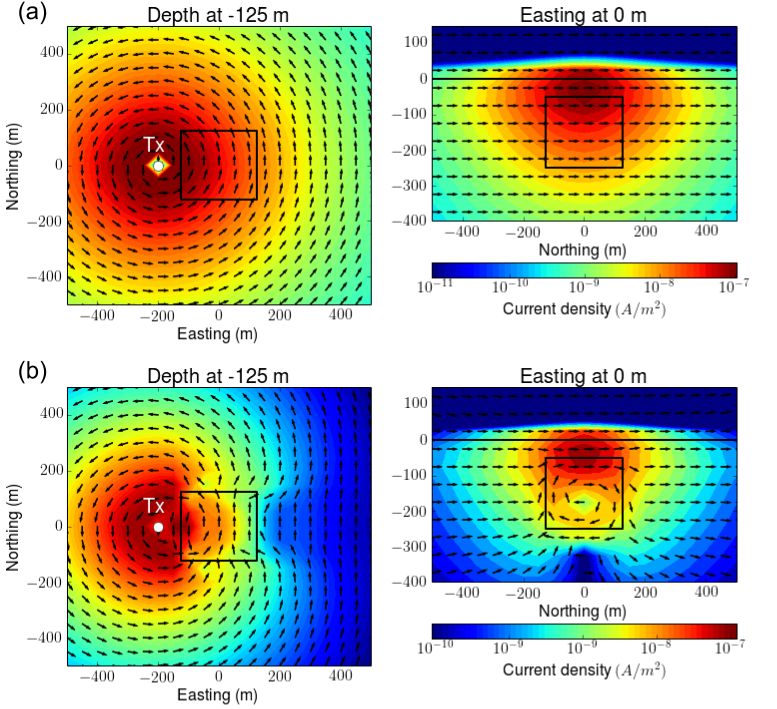
\includegraphics[width=1\textwidth]{figures/ReferenceCurrent.png} }
  \caption{Maps of reference currents: (a) canonical and (b) conductive models. Left and right panel show plan and section views at -125 m-depth and 0 m-easting, respectively. A transmitter is located at (-200 m, 0 m, 30 m). Black arrows and colored background indicate the direction and amplitude of the current, respectively. The black solid line outlines the boundary of chargeable body.}
  \label{F:ReferenceCurrent}
\end{figure}

\begin{figure}
  \figbox*{}{}{
  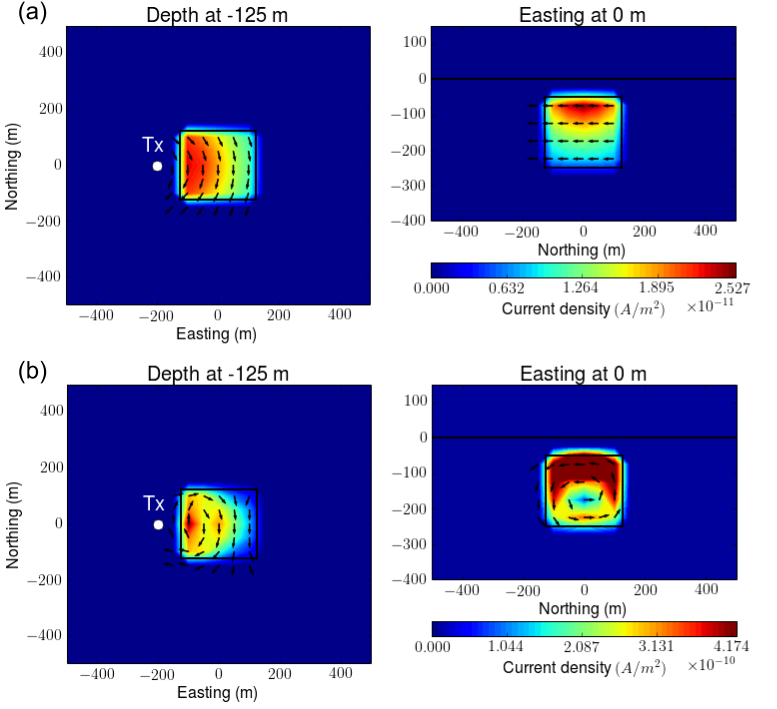
\includegraphics[width=1\textwidth]{figures/Polarizationcurrent_early.png} }
  \caption{Maps of polarization currents: (a) canonical and (b) conductive models at 0.86 ms. Left and right panels show plan and section views at -125 m-depth and 0 m-easting, respectively. A transmitter is located at (-200 m, 0 m, 30 m). Black arrows and shaded values indicate the direction and amplitude of the current, respectively. Black solid outlines boundary of the surface or the chargeable body.}
  \label{F:Polarizationcurrent_early}
\end{figure}

\begin{figure}
  \figbox*{}{}{
  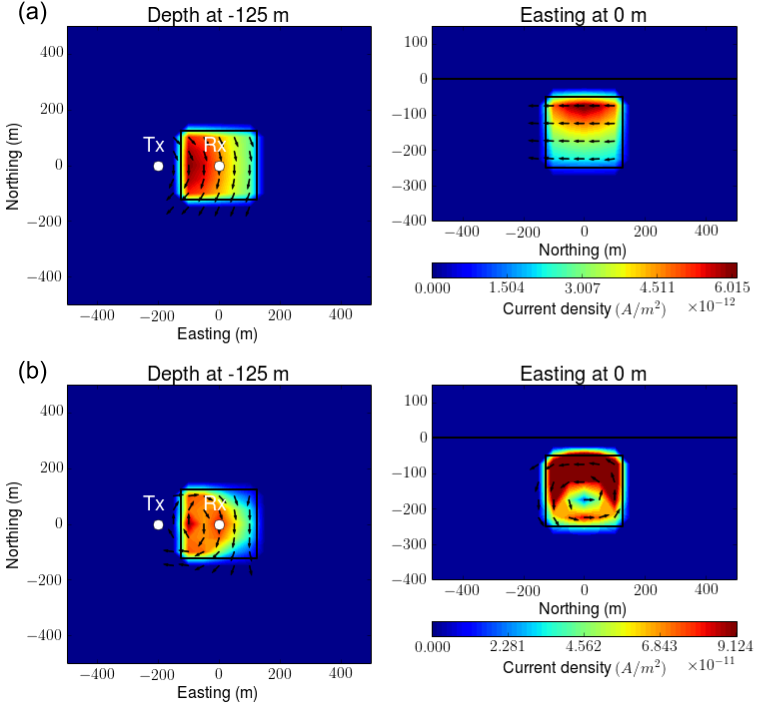
\includegraphics[width=1\textwidth]{figures/Polarizationcurrent_late.png} }
  \caption{Maps of polarization currents: (a) canonical and (b) conductive models at 6.7 ms. Left and right panels show plan and section views at -125 m-depth and 0 m-easting, respectively. A transmitter is located at (-200 m, 0 m, 30 m). Black arrows and shaded values indicate the direction and amplitude of the current, respectively. Black solid outlines boundary of the surface or the chargeable body.}
  \label{F:Polarizationcurrent_late}
\end{figure}
\clearpage

%%% ===========================================================================
%%% SUBSECTION
\subsection{IP currents}
The IP currents, as provided in equation (\ref{eq:IP_current}), are given as 
\begin{linenomath*}
\begin{equation}
  \j^{IP}=\siginf  \e^{IP} + \j^{pol}
\end{equation}
\end{linenomath*}
In most analyses, e.g. \cite{Smith1988a}, the term $\siginf \e^{IP}$ is neglected. We have included this term but with an approximation that $\e^{IP} \approx -\nabla \phi$  (equation \ref{eq: eip_approx}). Here we can investigate these approximations, and under what circumstances they hold. 

Using the forward modelling we can evaluate $e^{IP}$.
This field can be broken into galvanic and inductive parts using the Helmholtz decomposition: $\e=-\grad \phi-\vec{a}$ so that $\j^{IP} = \j^{pol} -\siginf \phi^{IP} - \siginf \vec{a}^{IP}$.
In our work we included the effects from the scalar potential but neglected entirely any contribution from the vector potential. 

We look at the contributions of each of these terms  for the three cases of canonical, conductive and resistive bodies. 
Figure ~\ref{F:IPcurrents_helmholtz_early} respectively show plan view maps of $\j^{pol}$, $-\siginf \vec{a}^{IP}$, and $-\siginf \phi^{IP}$ for (a) canonical, (b) conductive, and (c) resistive models at 0.86 ms. For all three cases the polarization currents have the greatest strength in the body and the strength of these currents is largest in the conductive body and smallest in the resistive body.
In all cases, the polarization currents are the largest contribution to $\j^{IP}$. 
The second column in Figure \ref{F:IPcurrents_helmholtz_early} is related to the scalar potential for the electric field or effectively to the galvanic currents. 
These exist both inside and outside the chargeable body.
Again, these are largest for the conductive body. 
We note that inside the body, these currents have a direction that is opposite to the polarization currents. 
The third column is associated with the vector potential for $\e^{IP}$ and is associated with vortex currents. 
The effects of these currents has not been included in our linearized approximations. These currents are quite small for the canonical and resistive models. They are most noticeable for the conductive model where their amplitude starts to be comparable to the galvanic portion. We note that the direction of the vortex currents inside the body is the same as for the galvanic currents and opposite to the polarization currents. 
We evaluate $\j^{IP} $ and its components at two locations in the body for conductive model. These are denoted by crosses in the figures.  For both points, the polarization currents have the greatest strength and vortex currents are smaller than the galvanic currents. At both locations the  IP current is smaller than the polarization current because galvanic and vortex IP currents are in the opposite direction compared to the polarization currents. The results are tabulated in Table \ref{T:DecompjIPcond}. 


The above figures provide insight about the three contributions to $\j^{IP}$ but of ultimate interest is the effect of these currents on the measured data. 
We therefore apply the Biot-Savart law to each current. It suffices to work with the conductive case. 
Figure ~\ref{F:DecompjIPcond} shows IP responses computed from the polarization current (stars), galvanic (rectangles) and inductive portions (circles) of the IP current. Here solid and empty markers show negative and positive signs, respectively. 
The polarization current has the major contribution to the IP response although it is larger than the true value. This overshoot is primarily negated by the galvanic portion of IP responses and further reduced because of the vortex currents. We notice that the contribution of the galvanic currents is generally larger than those due to the vortex currents except they are nearly equal near 0.4 ms. 
At 6.7 ms, the amplitude of the  IP response due to the polarization current is about 130 percent of the true one, while galvanic portion is 30 percent. 
These results show that the assumption of \cite{Smith1988a} is reasonable, but , a more accurate analysis shows that the contribution of the galvanic portion to the IP datum becomes more important at later times. 
The inductive portion of the IP responses  is small  compared to the galvanic portion except for the time before 0.2 ms, and hence ignoring this inductive portion is reasonable. 

\begin{figure}
  \figbox*{}{}{
  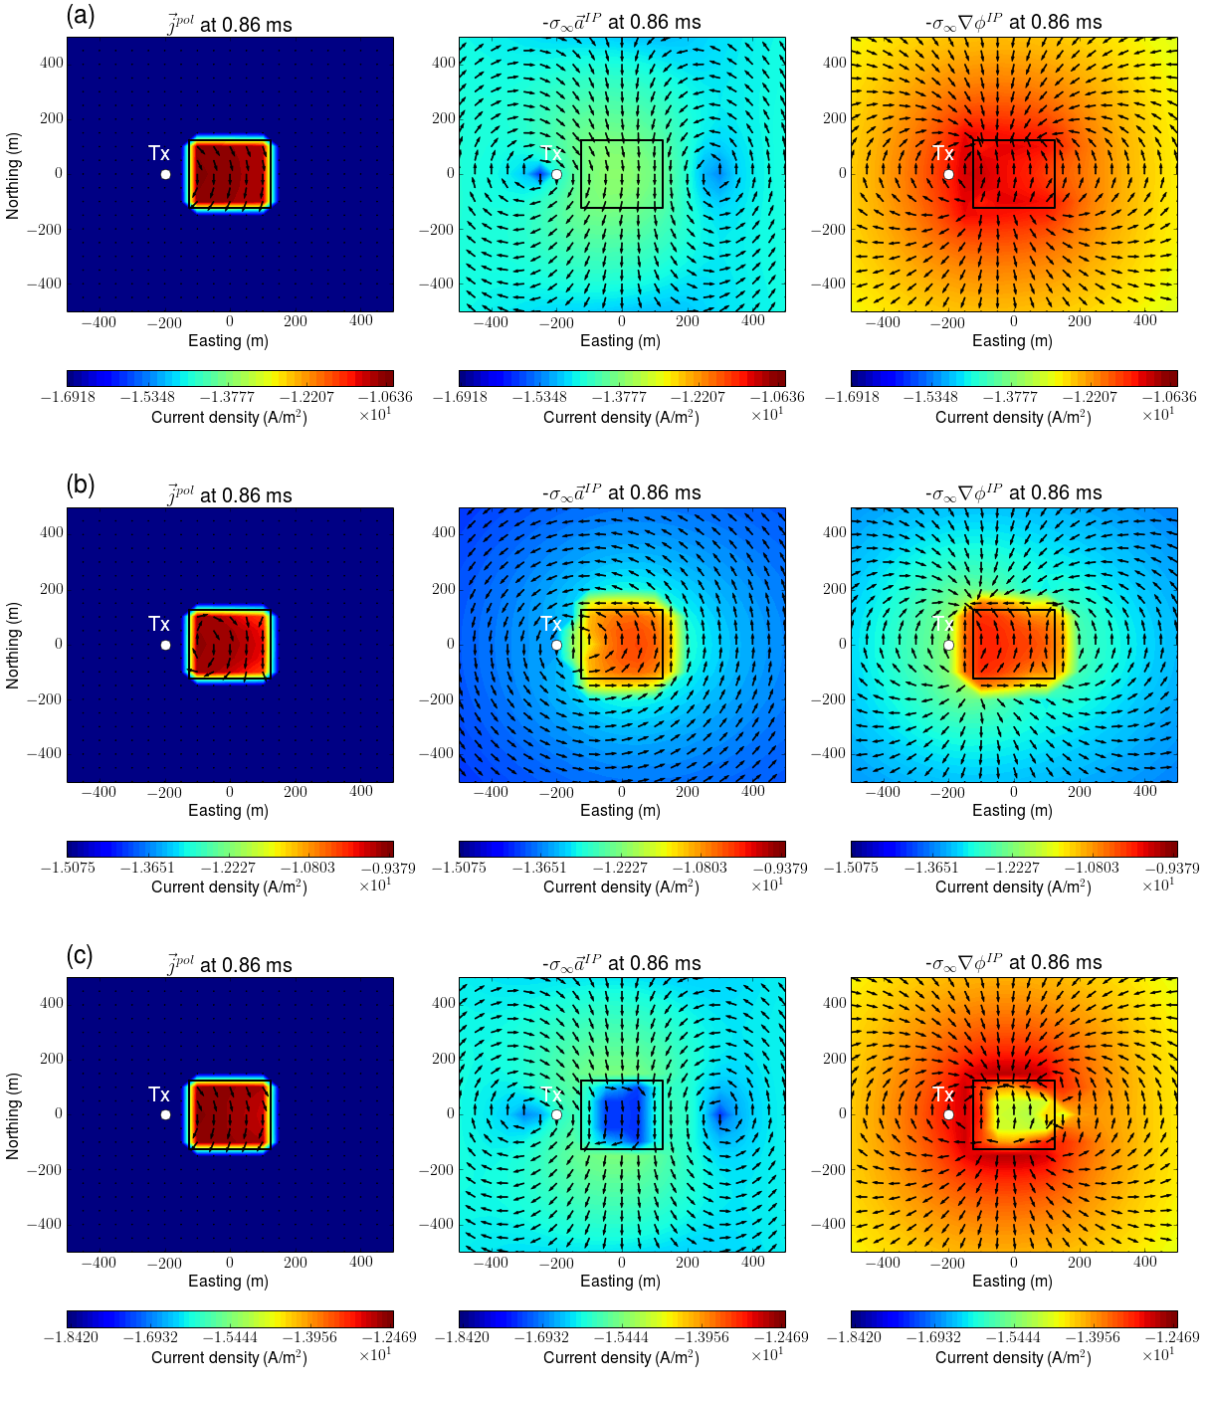
\includegraphics[width=1.\textwidth]{figures/IPcurrents_helmholtz_early.png} }
  \caption{Decomposition of the IP currents as $\j^{pol}$ (left panel), $-\siginf\grad \phi^{IP}$ (middle panel), and $-\siginf\vec{a}^{IP}$ (right panel) at 0.86 ms. Plan view maps of the currents at -125 m-depth are shown. (a) Canonical, (b) Conductive, and (c) Resistive cases. }
  \label{F:IPcurrents_helmholtz_early}
\end{figure}

\begin{figure}
  \figbox*{}{}{
  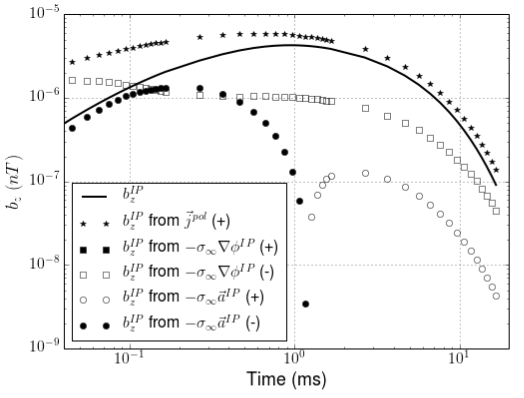
\includegraphics[width=1\textwidth]{figures/DecompjIPcond.png} }
  \caption{Comparisons of contributions of $\j^{pol}$, $-\siginf\grad \phi^{IP}$, and $-\siginf\vec{a}^{IP}$ to the observed IP responses. Solid line indicates true $b_z^{IP}$ responses. Stars, rectangles, and circles correspondingly indicate each IP response genrated by applying Biot-Savart law to $\j^{pol}$, $-\siginf\grad \phi^{IP}$, and $-\siginf\vec{a}^{IP}$. Empty and solid markers represent positive and negative values, respectively. }
  \label{F:DecompjIPcond}
\end{figure}

\begin{table}
 \caption{Amplitudes of decomposed IP currents at two marked points (crosses) shown in Figure ~\ref{F:DecompjIPcond}(b). Units in $A/m^2$}
 \label{T:DecompjIPcond}
 \begin{tabular}{@{}lccccc}
  Division & $| \j^{IP} |$ & $| \j^{pol} |$ & $| -\siginf\grad \phi^{IP} |$ & $| -\siginf\vec{a}^{IP} |$ \\
  Left  & $5.0\times 10^{-10}$ & $4.2\times 10^{-10}$ & $7.4\times 10^{-11}$ & $4.3\times 10^{-12}$ \\
  Right & $5.4\times 10^{-11}$ & $1.2\times 10^{-10}$ & $3.5\times 10^{-11}$ & $3.3\times 10^{-11}$ \\
 \end{tabular}
\end{table}

\clearpage


%%% ===========================================================================
%%% SUBSECTION
\subsection{Validations of linearization}
Forward modelling using our linear functional in equation (\ref{eq: dIP_lineareq}) requires that we have adequately estimated the IP currents and we can evaluate their response using the Biot-Savart law. To validate this we first compute approximate IP currents using equation (\ref{eq: jip_approx}), and first compare them with the true IP currents. It suffices to work with the conductive model which is the most challenging. Figure ~\ref{F:IPcurrent_PlanandSec_early} compares the true and approximate IP currents at 0.86 ms. The approximate IP currents match well, both in direction and amplitude, with the true IP currents both inside and outside the body. As shown in Figure ~\ref{F:IPcurrent_PlanandSec_late} the agreement improves as time increases.

We next test the validity of the computation of IP responses by using the our formulation of the Biot-Savart law. To do this we compute the ``true'' IP responses  by subtracting the fundamental response from the observations. We next compute the IP responses by evaluating the Biot-Savart law with the true IP currents shown in Figure ~\ref{F:IPcurrent_PlanandSec_late}(a). As shown in Figure ~\ref{F:True_vs_approx_IPresp} the agreement between these responses is very good after 0.01 ms. This validates the use of the Biot-Savart law (equation (\ref{eq: BiotbIP_approx})). Lastly, we want to compare responses, evaluated through the Biot Savart law, using our approximated IP currents (Figure ~\ref{F:IPcurrent_PlanandSec_late}(b)).
The results are shown in Figure ~\ref{F:True_vs_approx_IPresp}. The responses obtained from using our approximate currents have lower amplitude and differ by 33 percent at the extreme. The difference decreases with increasing time. Overall the two curves are in reasonable agreement, thus validating our linearized forward modeling equation (\ref{eq: dIP_lineareq}).

The same analysis as above was carried out for the canonical and resistive models. As shown in  Figure ~\ref{F:True_vs_approx_IPresp} the agreement is further improved. We note however, that despite the fact that our linear functional reasonably explains $\dip$ data for the resistive case, the IP signals are so small that we likely can’t distinguish them in practise.

\begin{figure}
  \figbox*{}{}{
  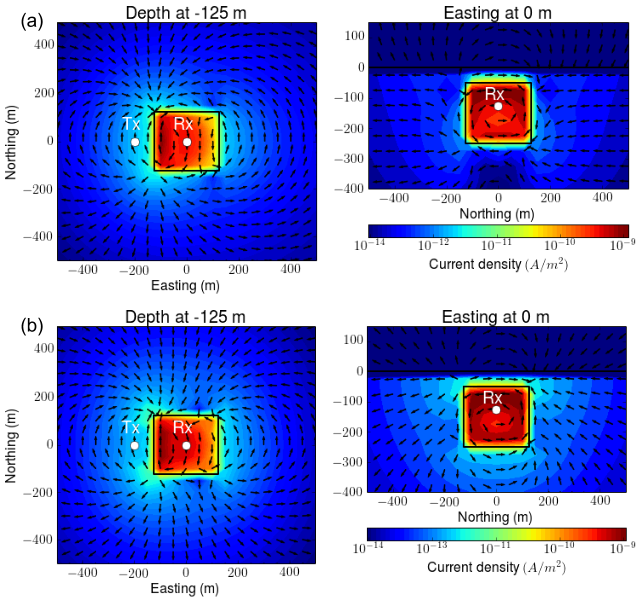
\includegraphics[width=1\textwidth]{figures/IPcurrent_PlanandSec_early.png} }
  \caption{Interpolated maps of (a) true and (b) approximate IP currents at 0.86 ms. Left and right columns show plan and section view maps at -125 m-depth and 0 m-easting, respectively. }
  \label{F:IPcurrent_PlanandSec_early}
\end{figure}

\begin{figure}
  \figbox*{}{}{
  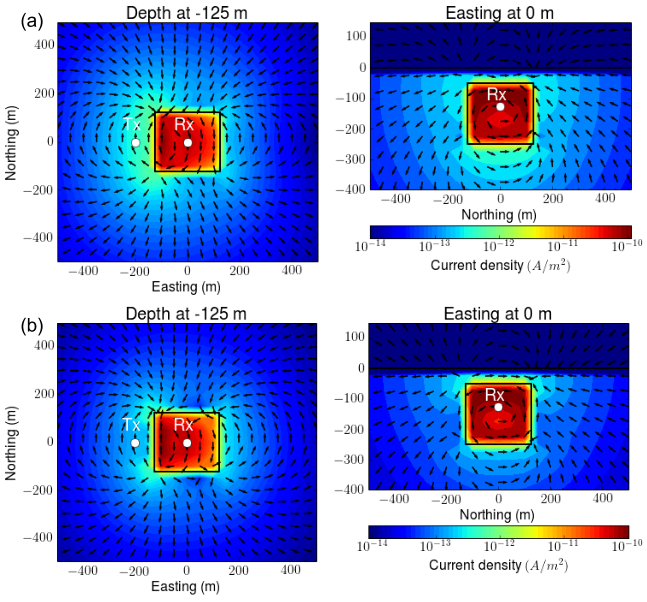
\includegraphics[width=1\textwidth]{figures/IPcurrent_PlanandSec_late.png} }
  \caption{Interpolated maps of (a) true and (b) approximate IP currents at 6.7 ms. Left and right columns show plan and section view maps at -125 m-depth and 0 m-easting, respectively. }
  \label{F:IPcurrent_PlanandSec_late}
\end{figure}

\begin{figure}
  \figbox*{}{}{
  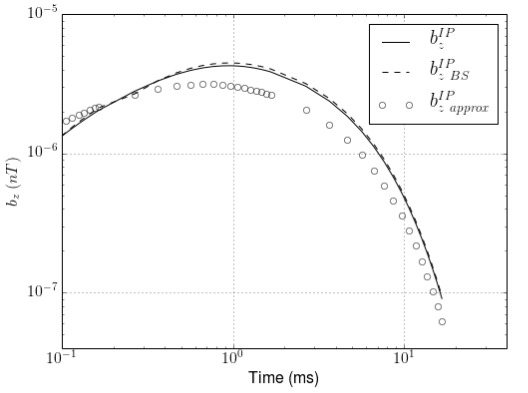
\includegraphics[width=1\textwidth]{figures/True_vs_approx_IPresp.png} }
  \caption{Comparison of true and approximate IP respones ($b_z^{IP}$). Black, blue, and red color respectively indicate canonical, conductive, and resistive cases. Solid lines indicate true $b_z^{IP}$ computed by subtraction process. The stars are the application of Biot-Savart to true IP current and generate $b_{z \ BS}^{IP}$. Empty circles show our approximate $b_{z \  approx}^{IP}$ response. }
  \label{F:True_vs_approx_IPresp}
\end{figure}
\clearpage


%%% ===========================================================================
%%% SUBSECTION
\subsection{Effective pseudo-chargeability for ATEM data}
\label{subsection: Effective pseudo-chargeability for ATEM data}

In Section \ref{subsection: Effective pseudo-chargeability for ATEM data} we showed how to define an effective chargeability when we have multi-transmitters. For each pixel we have
equation: 
\begin{equation}
  \peta_i(t) = \peta_i^I(t) \otimes  w_i^e(t),
\end{equation}
where $\peta_i^I(t)$ is the intrinsic chargeability associated with an individual pixel. The effective time history of the electric field, $w_i^e(t)$ is a linear combination of the fundamental electric fields due to the individual transmitters. We can calculate $w_i^e(t)$ and carry out the convolution to evaluate the effective pseudo-chargeability. The IP data can then be forward modelled suing eq. (\ref{eq: dIP_lineareq}).We can test eq. (\ref{eq: dipeff_kthTx}) by comparing results with the true IP data obtained via forward modelling. It is only necessary to apply this to the conductive model. 

The evaluation of the effective pseudo-chargeability is carried out on  a cell by cell basis. For each cell  we  first evaluate $w^e(t)$ (equation (\ref{eq: we_eff})). This requires calculating normalized weights shown in equation (\ref{eq: normalized_weights}). 
Figure ~\ref{F:NormalizedWeights} shows these weights at a single pixel located at (0 m,0 m,-75 m). These decay away from the pixel because of the decay of the sensitivity functions.  The $w^e(t)$, evaluated using equation (\ref{eq: we_eff}), is shown in Figure ~\ref{F:AveragedWe} (solid line). The $\hat{w}(t)$ (dashed lines) for each transmitter are also shown. The $w^e(t)$ is dominantly affected by the $\hat{w}(t)$ at the center transmitter location (solid circles). The $w^e(t)$ is convolved  with  $\peta^I(t)$ to compute the effective $\peta(t)$ for that cell. When this is carried out for each cell then the approximate IP responses can be computed using linear functional (equation (\ref{eq: dIP_lineareq})). These can be compared with the true IP responses. 
Figure ~\ref{F:EquivPeta_True_Approx} show the comparisons at a time of 0.86 ms. The images are nearly identical in shape but the approximate IP responses are nearly a factor of two lower than the true values. This is not entirely unexpected. A similar effect was observed for IP responses for a single transmitter shown in Figure ~\ref{F:True_vs_approx_IPresp}. At 0.86 ms, the approximate value was about 70 percent of the true $\dip$. These results seem to be a worst case scenario. The discrepancy for a conductive body lessens as time increases and analyses for the canonical and resistive bodies shows that the approximate and true IP data are in very good agreement. 

\begin{figure}
  \figbox*{}{}{
  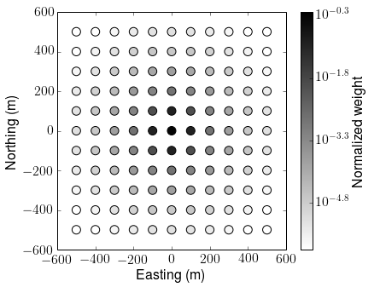
\includegraphics[width=1.\textwidth]{figures/NormalizedWeights.png} }
  \caption{Normalized weights for the conductive case for all trasmitter locations. A single pixel located at (0 m, 0 m, -75 m) is used. }
  \label{F:NormalizedWeights}
\end{figure}

\begin{figure}
  \figbox*{}{}{
  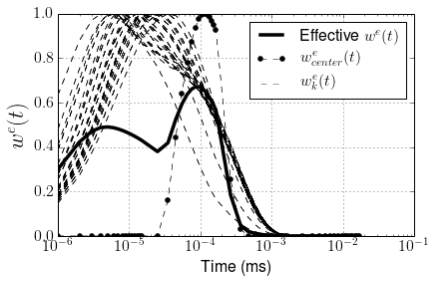
\includegraphics[width=1.\textwidth]{figures/AveragedWe.png} }
  \caption{Time decays of $w^e(t)$ and $\hat{w}(t)$ for the conductive case. A single pixel located at (0 m, 0 m, -75 m) is used. Solid line and dashed lines correspond to $w^e(t)$ and $\hat{w}_k(t)$ for all transmitters ($k=1,\ \ldots,\ nTx$); $\hat{w}_k$ at the center transmitter located at (0 m, 0 m, 30 m) is marked as solid circles. }
  \label{F:AveragedWe}
\end{figure}
\clearpage

\begin{figure}
  \figbox*{}{}{
  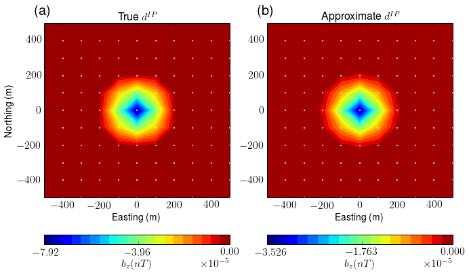
\includegraphics[width=1.\textwidth]{figures/EquivPeta_True_Approx.png} }
  \caption{Comparison of true and approximate $b_z^{IP}$ responses at 0.86 ms on plan view map. }
  \label{F:EquivPeta_True_Approx}
\end{figure}
\clearpage

%%% ===========================================================================
%%% SUBSECTION
\subsection{3D IP inversions}
Using our linearized sensitivity, we now proceed with 3D IP inversion, which recovers a pseudo-chargeability given by equation (\ref{eq: dIP_lineareq}). 
We limit our attention to the conductive case. For the computation of the sensitivity we use the true conductivity ($\siginf$) and then invert data at successive time channels and recover 3D pseudo-chargeability at multiple times. 
Our 3D inversion is based upon \cite[]{doug1994,Li2000}, and it requires some choices for inversion parameters. 

For data uncertainties, we used one percent of the maximum amplitude of the observed data (0.01$max(|\mathbf{d}^{obs}|)$). Coefficients for smallness and smoothness are set to $\alpha_s=10^{-5}$ and $\alpha_x=\alpha_y=\alpha_z=1$, respectively. The reference model is zero and we also applied a depth weighting. 
The need for a depth weighting arises because the sensitivity function $J$ is primarily controlled by a $1/r^3$ decay associated with the Biot-Savart kernels.  Thus an ATEM data set is not unlike commonly acquired  magnetic data where it is well established that a depth weighting is required to image objects at depth. The following example illustrates this. 

We first generate IP responses at a single time using the linear functional by assuming that the pseudo-chargeability is unity inside the body and zero outside, as shown in  Figure \ref{F:Depthweight}(a). 
Figure \ref{F:Depthweight}(b) shows the recovered pseudo-chargeability without depth weighting. 
The recovered anomalous pseudo-chargeability is concentrated  near the surface and the magnitude of the pseudo-chargeability is underestimated; it is $\sim$0.2 rather than unity. 
By using the depth weighting shown in equation (\ref{eq: weight_mat}),  the IP body is imaged closer to its true depth (Figure \ref{F:Depthweight}(b)). 
Also, the magnitude of the recovered pseudo-chargeability ($\sim$0.6) is closer to the true value than the result without depth weighting. 
Based on this analysis, we use the same depth weighting for our  following examples. 

\begin{figure}
  \figbox*{}{}{
  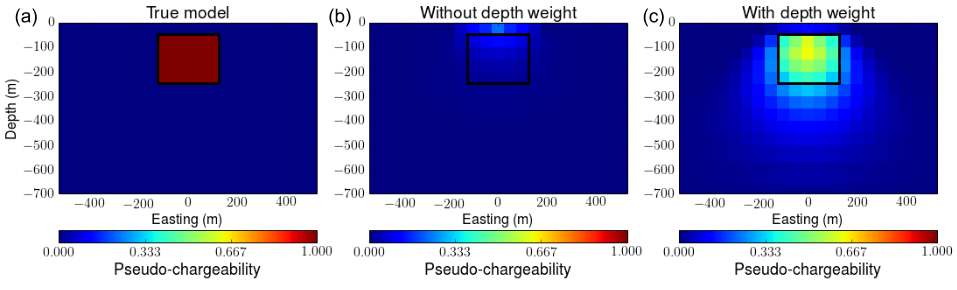
\includegraphics[width=1.\textwidth]{figures/Depthweight.png} }
  \caption{Effect of depth weight in 3D IP inversion. (a) True pseudo-chargeability model on vertical section at 0 m-northing. Recovered pseudo-chargeability models (b) without depth weight and (c) with depth weight.}
  \label{F:Depthweight}
\end{figure}
\clearpage

%%% ===========================================================================
\subsubsection{Incorrect conductivity}
The background conductivity $\siginf$ plays a central role in our analysis. It is used in the EM decoupling process and it is also needed to compute the linearized sensitivities for inversion. Since we need to estimate $\siginf$, usually through the inversion of EM survey data, it will never be correct. Here we explore some effects of an incorrect conductivity but  the consequences are problem dependent.

We return to our conductive block in a halfspace and evaluate the $\dip$ data when the background is the true value ($\sigma_1 = 10^{-3}$ S/m) as well as a factor of two too large (2$\times10^{-3}$ S/m) and a factor of two too small (5$\times10^{-4}$ S/m). The data along a survey line are plotted in Figure \ref{F:Reg_IPresp}.

We invert these three IP responses, and provide sections of the recovered pseudo-chargeability at 0 m-northing. 
Figure \ref{F:Regional_IPInv}(a), (b) and (c) correspondingly show the recovered pseudo-chargeability when the conductivity is: the true value, too high, or too low.  
With the correct conductivity the geometry of the IP body is reasonably recovered. 
When the conductivity is too high, the $\dip$ have a negative bias that results in larger pseudo-chargeabilities and positive-valued artifacts near the IP body (Figure \ref{F:Regional_IPInv}(b)).  
When the conductivity is too small, the IP data have a positive bias and this produces  negative-valued artifacts near the IP body (Figure \ref{F:Regional_IPInv}(c)). However, based on the  definition of the pseudo-chargeability shown in equation (\ref{eq: petaeff}), the sign of the pseudo-chargeability should be positive. By incorporating positivity as a constraint in the inversion, re-inverting the IP data having a positive bias we obtain the result in  Figure \ref{F:Regional_IPInv}(d).  This is a much better result than Figure \ref{F:Regional_IPInv}(c)  and comparison of the observed and predicted data for this case shown in Figure \ref{F:Reg_obspred} clearly shows how this constraint prevents the fitting of positive residual fields. We shall use this positivity  constraint for our following 3D IP inversion examples. 

The background conductivity is also needed when computing the sensitivity function, since we need the reference electric field, which is dependent on conductivity. 
An incorrect conductivity will affect the sensitivity function as well. 
In order to test this, we compute the sensitivity  matrix using a half-space conductivity model ($\siginf = \sigma_1$). 
Figure \ref{F:True_vs_approx_sensitivity} compares the recovered pseudo-chargeability from the 3D IP inversion of the IP datum at 0.86 ms with the true and incorrect sensitivity function using half-space conductivity. 
There is not a large difference between the two inversions  which suggests that an approximate conductivity may still provide sensitivities that are adequate for inversion. This parallels results from EIP where even an approximate conductivity can still yield good results when inverting the data. Thus there is some robustness in our sensitivity function with respect to an  incorrect conductivity and even if we  not have an accurate 3D conductivity model we can still apply our 3D IP inversion using half-space conductivity so long as the ATEM data includes distinctive IP response such as negative transients.

\begin{figure}
  \figbox*{}{}{
  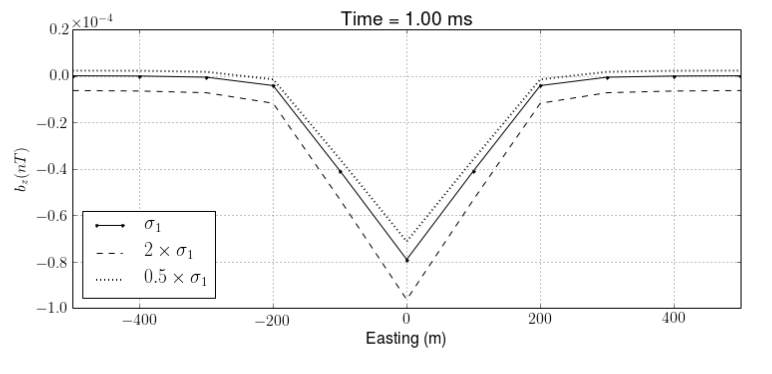
\includegraphics[width=1.\textwidth]{figures/Reg_IPresp.png} }
  \caption{IP responses on a profile line at 0 m-northing.  IP responses are computed from perturbed $\siginf$ models. Half-space conductivity ($\sigma_1$) is perturbed two times higher or less resulting in overestimated (dotted line) and underestimated (dashed line) IP respones. Solid line shows the true IP response. }
  \label{F:Reg_IPresp}
\end{figure}

\begin{figure}
  \figbox*{}{}{
  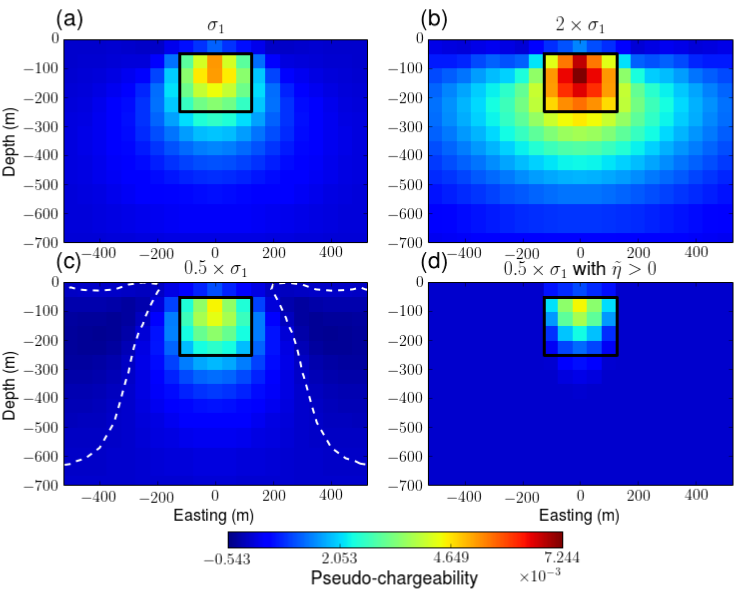
\includegraphics[width=1.\textwidth]{figures/Regional_IPInv.png} }
  \caption{Recovered pseudo-chargeability sections from 3D IP inversions at 0 m-northing. (a) $\dip$ with true $\sigma_1$. (b) $\dip$ with 2$\times \sigma_1$. (c) $\dip$ with 0.5$\times \sigma_1$. (d) $\dip$ with 0.5$\times \sigma_1$ and the positivity constraint on the pseudo-chargeability. White dashed lines contour zero-crossing lines.}
  \label{F:Regional_IPInv}
\end{figure}

\begin{figure}
  \figbox*{}{}{
  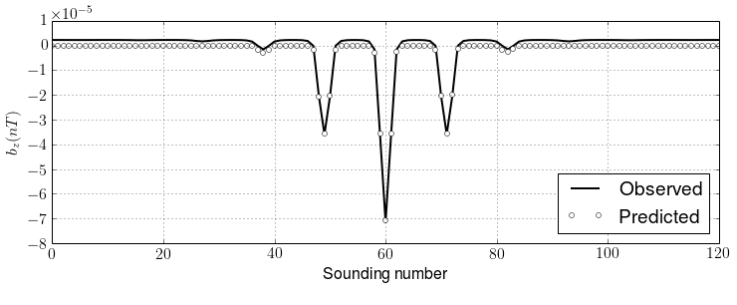
\includegraphics[width=1.\textwidth]{figures/Reg_obspred.png} }
  \caption{Comparison of the observed (solid line) and predicted (empty circles) data. $\dip$ response was generated with underestimated half-space conductivity (0.5$\times \sigma_1$). The positivity constraint was used the 3D IP inversion.}
  \label{F:Reg_obspred}
\end{figure}

\begin{figure}
  \figbox*{}{}{
  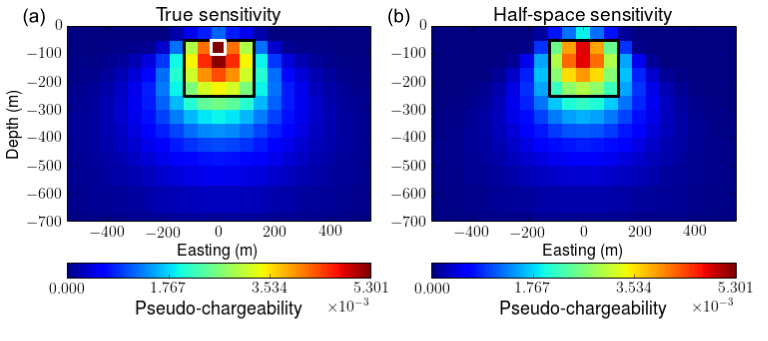
\includegraphics[width=1.\textwidth]{figures/True_vs_approx_sensitivity.png} }
  \caption{Recovered pseudo-chargeabilty sections from the 3D IP inversions at 0 m-northing.  (a) True and (b) incorrect $\siginf$ is used to compute sensitivity function. For the incorrect sensitivity we used half-space conductivity ($\sigma_1$).}
  \label{F:True_vs_approx_sensitivity}
\end{figure}
\clearpage

%%% ===========================================================================
\subsubsection{Extracting intrinsic IP parameters}
By applying our inversion to each time channel of $\dip$ data separately, we can recover 3D distributions of pseudo-chargeability at multiple times. 
The pseudo-chargeability at each time carries different information about the state of polarization and we can use these to recover information about intrinsic IP parameters. 
Diverse time-dependent conductivity models such Cole-Cole model and stretched-exponential can be used for this interpretation.
We use the Cole-Cole model with $c=1$. 
We parametrize pseudo-chargeability at a single pixel in terms of chargeability and time constant as described in Section \ref{section: extract_intrinsicIP}, and solve a small inverse problem. This parallels \cite[]{Yuval1997,Hordt2006}.

As an example, we use the conductive and chargeable block presented in the previous section and invert 14 time channels of data ranging from 1-10 ms.  The EM data are forward modelled using xxxx and the true $\siginf$ model is used  to evaluate the IP datum compute the sensitivity function. The recovered pseudo-chargeability from one of the 14 inversions is shown in Figure \ref{F:True_vs_approx_sensitivity}a. In that pseudo-chargeability model, we choose cells having greater pseudo-chargeability value than 0.001, and then carry out the nonlinear inversion to estimate the time constant ($\tau$) and chargeability ($\eta$) of each cell separately. The forward kernel for this inversion is shown in equation (\ref{eq: pseudochargeability_petaI}), which requires $w^e(t)$. 
The $w^e(t)$ for a pixel in the block is shown in Figure \ref{F:AveragedWe}.

Figure ~\ref{F:EtaTauSection}a and b correspondingly show the estimated time constants and chargeability as section maps.
The estimated time constants show good agreement with the true value $\tau= 0.005$. 
There is less agreement about chargeability for which the true value is $\eta=0.2$. Recovered values range from about 0.04-0.2 so most values are underestimated. 
In Figure \ref{F:IntrinsicIP}, we also provide time decays of the observed and predicted pseudo-chargeabilities at a single pixel marked as a black empty rectangle in Figure ~\ref{F:EtaTauSection}. The estimated time constant ($\tau_{est}$) and chargeability ($\eta_{est}$) for this pixel are 0.0046 and 0.09, respectively. 
These results imply there is greater  stability on recovering time constant than on recovering chargeability with our approach. Again, similar experiments were carried through for the canonical and resistive bodies and the conclusions were also that the time constant was adequately recovered with better fidelity than was the intrinsic chargeability.  

\begin{figure}
  \figbox*{}{}{
  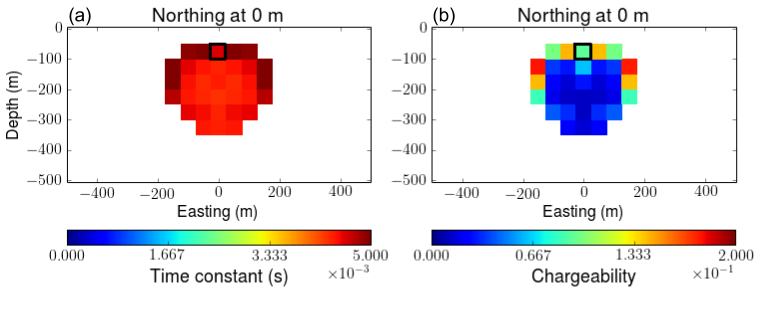
\includegraphics[width=1.\textwidth]{figures/EtaTauSection.png} }
  \caption{Section views of recovered (a) time constant and (b) chargeability. Any region where the peudo-chargeabiliy shown in Figure ~\ref{F:True_vs_approx_sensitivity}a is smaller that 0.001 is ignored this analysis, and blanked.}
  \label{F:EtaTauSection}
\end{figure}

\begin{figure}
  \figbox*{}{}{
  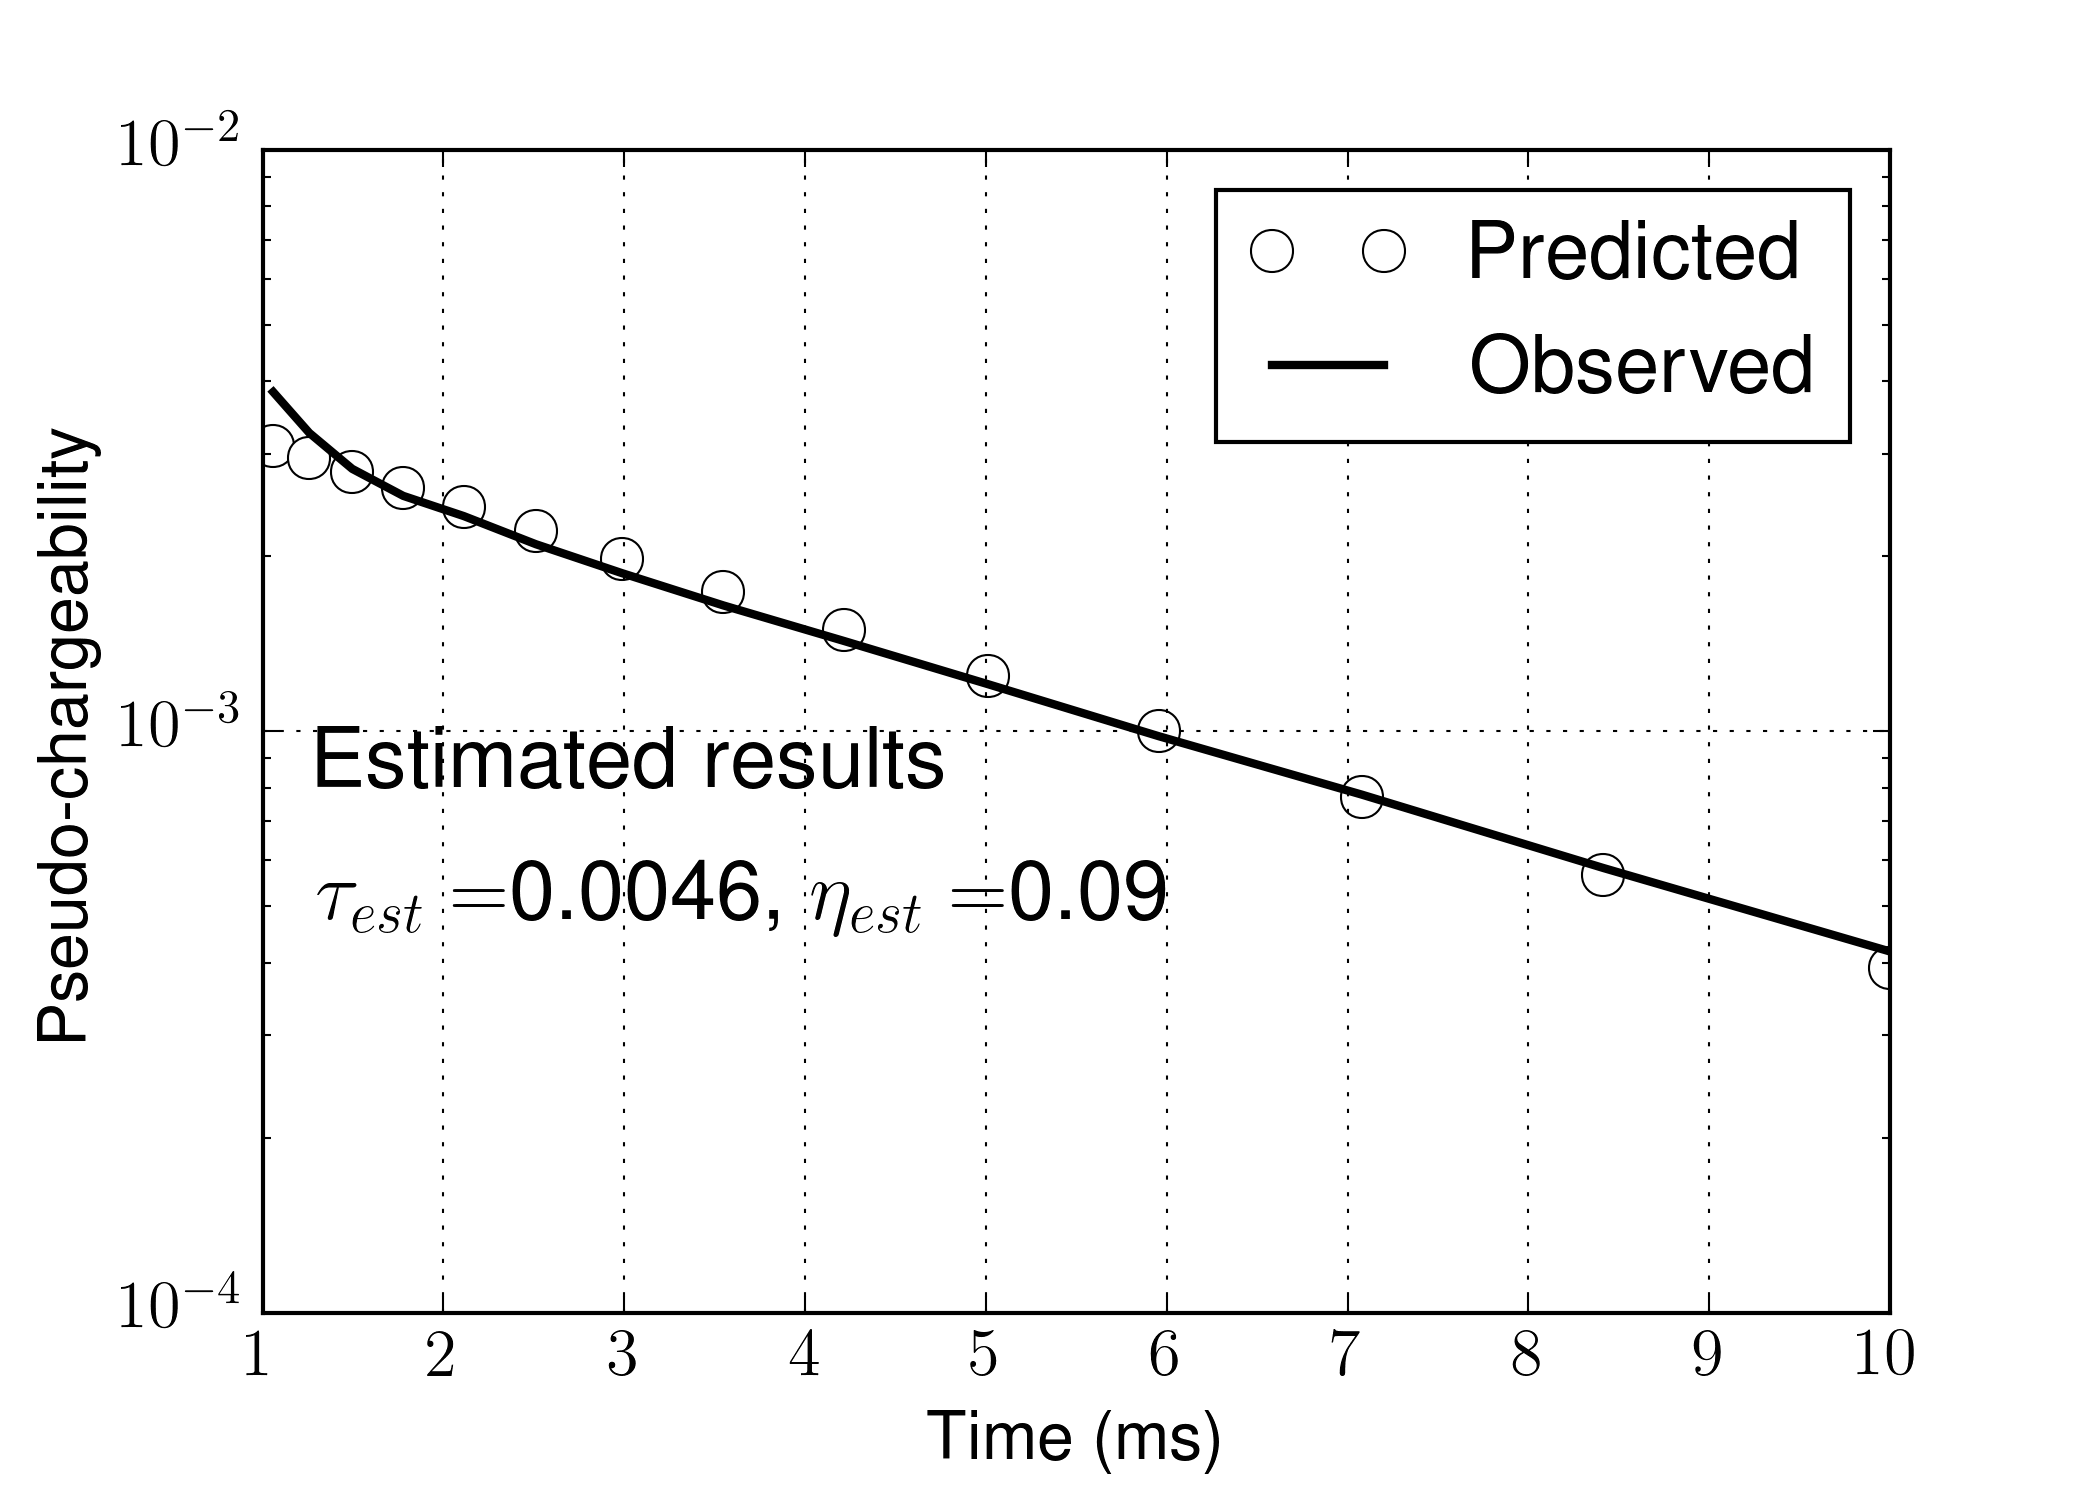
\includegraphics[width=1.\textwidth]{figures/IntrinsicIP.png} }
  \caption{Comparisons of the observed and predicted pseudo-chargeability at a single pixel in a chargeable body. 
  Empty and solid circles indicate predicted pseudo-chargeabilities using two different $w^e_{avg}(t)$ for the choices of normalized weights: a single cell and all cells in a chargeable block, respectively. Estimated time constant and chargeability for each inversion are expressed as $\tau_{est}$ and $\eta_{est}$, respectively.}
  \label{F:IntrinsicIP}
\end{figure}
\clearpage

%% =============================================================================
%% Section. Conclusions
%% =============================================================================
\section{Conclusions}
In this paper, we have introduced a procedure for recovering IP from TEM data with inductive sources.  Three main steps are required: 1) subtraction of the fundamental responses from the observations to generate IP data, 2) linearization of the IP responses as a function of the pseudo-chargeability, and 3) restoration of 3D pseudo-chargeability at multiple times, and further interpretation of the pseudo-chargeability to extract intrinsic IP parameters like Cole-Cole model. We used the ATEM survey to test our IP inversion procedure.

The first step requires that we have a good estimate for the background conductivity $\siginf$. This is important for two reasons. It is first used to generate the fundamental fields that are subtracted from the observations to produce the IP data. This conductivity is also needed to compute the sensitivities for our linear relationship between the IP data and pseudo-chargeability. To construct $\siginf$ for our work here we used the early time data that was felt to be uncontaminated with significant IP responses and inverted those with our 3D algorithms. For the mid-time data, subtraction of the fundamental responses from the observations revealed negative data even though the observations had been positive. At very late times however, this subtraction process was not necessary since the EM fields had sufficiently decayed. Maps of the $d^{IP}$ can, in themselves, be a useful processing tool for anomaly hunting.

The second item, linearization of the IP responses with respect to a pseudo-chargeability, required that a number of assumptions  be made. This pseudo-chargeability is defined as the ratio of the polarization current to a reference current. Unlike the EIP case, the electric fields for an inductive source do not achieve steady-state and hence neither do the polarization currents. This fundamental difference is addressed by evaluating the fundamental fields at each location in the earth and generating a reference electric field that has the direction and magnitude of the field at time when the fundamental field, which is responsible for charging the earth, reaches its maximum value. The pseudo-chargeability at a point in the earth thus depends upon the intrinsic chargeability, the reference electric field and the time history of the fundamental electric field. The situation becomes more complicated when data from many transmitters are to be inverted simultaneously because the time history of the electric field at a point in the earth is different for each transmitter. We handle this by defining an effective pseudo-chargeability and an associated reference electric field that accommodates, in a least squares fashion, the effects of all transmitters acting on a single cell.

To have confidence in when, and under what circumstances, our approximations are sufficiently valid, we proceed with a number of rigorous tests. First we introduce 3 test models which are respectively a chargeable block in a halfspace. The block can be conductive, canonical, or resistive with respect to the background. Our evaluations show that: 
(a) our choice of reference electric field and its time history produces a good estimate of the polarization currents;
(b) the IP currents are dominated by the polarization currents, which is an assumption that is often made. However, the galvanic and vortex currents arising from the scalar and vector potentials in the Helmholtz decomposition of $\ e^{IP}$ can be significant in some circumstances. They both oppose the direction of the polarization currents in the body. In our work we have included the galvanic currents and neglected the vortex currents which are almost always smaller than the galvanic currents.
(c) Evaluating the IP responses using the Biot-Savart law provides accurate results.
(d) With our approximate IP currents, the predicted responses are in reasonably good agreement with those from the true models although they are underestimated for highly conductive example. These results lead us to infer that our linearized formulation $d^{IP}(t)=J\peta(t)$ is a viable representation for the forward modelling at late times when  the IP effect is substantial compared to the EM effects which will occur in the discharging phase. 
(e) For the multi-transmitter case we derived an effective pseudo-chargeability, which is a linear combination of the pseudo-chargeability of each transmitter. These were forward modelled with the linearized formulation and compared to the true responses. The computed responses showed the same shape; the values were underestimated for the conductive model but were almost identical for the canonical and resistive models.  

The third component is the 3D inversion of the IP data using the linearized formulation to recover an effective pseudo-chargeability for each cell. ATEM data have only one receiver for each transmitter and a data map at a single time channel is essentially a potential field. The data do not have intrinsic resolving power and hence, as in magnetics or gravity inversions, we attempt to counteract this by introducing a depth weighting.  When this is done, our 3D IP inversion recovers a reasonable geometric shape and location of the chargeable body but the amplitude is underestimated. An incorrect $\siginf$ has two effects in the inversion. Firstly it can generates errors in the $d^{IP}$ data because the fundamental field, which is subtracted from the observations, is incorrect. To obtain insight we looked at the effects when the $\sigma_{est}$ was too low or two high. This respectively yielded positive or negative residual fields in the IP response. A positivity constraint on the pseudo-chargeability (similar to that used in EIP surveys) greatly ameleorated the effects of the positive residuals. The other avenue by which an incorrect $\siginf$ can affect the inversion is through the sensitivity matrix $J$. We showed that even with a poor sensitivity function, computed using half-space conductivity model, we recovered important information of the chargeable body such as geometric shape and location. Individual inversion are carried out at all time channels. The result is a recovered pseudo-chargeability as a function of time for each pixel in the earth. The pseudo-chargeability for pixels that had significant chargeability were subsequently fit to a Cole-Cole model to estimate $\tau$ and $\eta$ by assuming $c=1$. The estimated $\tau$ was close to the true value whereas $\eta$ was underestimated and less robust. This suggests that there is possibility to extract intrinsic IP parameters from the recovered pseudo-chargeability from ATEM surveys.  

Our IP inversion procedure provides a framework for recovering IP information from inductive source EM surveys and in particular from ATEM surveys that are commonly flown. Our examples show: (a)  that the horizontal location of a target body can be well recovered; (b) the overall geometry might be recovered but much of that inference requires a depth weighting to be included; (c)  we can recover estimates of intrinsic $\tau$ and $\eta$ that may be useful for distinguishing between two chargeable targets. Our procedure depends on having a good estimate for the background conductivity and this aspect this should be carefully investigated in future practical applications of our inversion methodology.  Other areas for follow-up research include depth resolution of airborne IP and robust inversion methodology to extract intrinsic IP parameters from TEM data. 
Lastly, our numerical examples  only treated the ATEM survey, but the procedure is applicable to other types of inductive source TEM survey such as Large-loop TEM with many receivers. There will be details that need to be addressed for those applications but the work presented here provides the  fundamental backgrounds for those future studies whose goal is to extract some information about polarization from an inductive time domain system. 


% =======================================================================
% SECTION (Appendix)
% =======================================================================
\appendix
%% ===========================================================================
%% SUBSECTION
\section{Discretization of steady-state Maxwell's equations}
\label{section:maxwell_discrete}
As shwon equation (\ref{eq: phiIPapprox_general}), computation of our linearized kernel requires solving steady-state Maxwell's equations. 
We discretize this system using mimetic finite volume (FV) method with weak formulation \cite[]{Eldadbook}. 
For the discretization, we assume that the electric field $\e$ is discretized by grid function $\de$ on cell edges and magnetic flux density $\b$ is discretized by grid fuction $\db$ on cell faces. 
Electrical potential $\phi$ is discretized by grid fucntion  $\phi$ on cell nodes. For clear representation of the derivation, recall Maxwell's equations in steady state as
\begin{align}
  \j = \siginf\e = -\siginf\grad \phi, \\
  -\div \j = \div \j_s, \\
  \j\big|_{\partial \Omega}\cdot\hat{n} = 0,
  \label{eq:DCBCneumann}
\end{align}
where $\partial \Omega$ indicates boundary surface of the system and $\hat{n}$ is the normal vector of the boundary surface. Weak form of those equations can be written as
\begin{align}
  (\j, \vec{w}) + (\siginf \grad \phi, \vec{w}) = 0, \\
  -(\j, \grad \psi) = (\j_s, \grad \psi).
\end{align}
The inner products $(\j, \vec{w})$, $(\siginf \grad \phi, \vec{w})$,  $(\j, \grad \psi)$ and $(\j_s, \grad \psi)$ are edge based products. Here we define the inner product as
\begin{linenomath*}
\begin{equation}
  (\vec{a}, \vec{b}) = \int_{\Omega} \vec{a}\cdot\vec{b} dv,
\end{equation}
\end{linenomath*}
where $\Omega$ is the volume of the system. By discretizing $\grad$ operator and the inner product in space, we obtain
\begin{linenomath*}
\begin{equation}
  \Me\dj + \MeSigInf\dgrad\boldsymbol{\phi} = 0,
  \label{eq:DCdisceq1}
\end{equation}
\end{linenomath*}
\begin{linenomath*}
\begin{equation}
  -\dgrad^T \Me\dj = \dgrad^T \Me\dj_s,
  \label{eq:DCdisceq2}
\end{equation}
\end{linenomath*}
where $\mathbf{M}^e_i$ is the mass matrices, which discretize the edge based inner product (\cite[]{Eldadbook}). This inner products are defined  as
\begin{align}
  \mathbf{M}^e_i = \diag(\Ace^T\diag(\vol)\mathbf{i}).
\end{align}
Here, $\mathbf{i}$ indicates a grid function on cell center like $\siginf$, and $\vol$ is the grid function for the cell volume. The averaging matrix $\Ace$ averages discrete function defined on the edges to the cell center. The mass matrix $\Me$ without subscript $i$ indicates that $\mathbf{i}$ is equal to the identity column vector of which all elements are one. By substituting equation (\ref{eq:DCdisceq1}) to (\ref{eq:DCdisceq2}), we have
\begin{linenomath*}
\begin{equation}
  \A_{\siginf}\boldsymbol{\phi} = \mathbf{rhs}^{DC},
  \label{eq:DCdiscLin}
\end{equation}
\end{linenomath*}
where $\A_{\siginf} = \dgrad^T \MeSigInf\dgrad$ and $\mathbf{rhs}^{DC} = \dgrad^T \Me\dj_s$. 

%% ===========================================================================
%% SUBSECTION
\section{Discretization of the linearized kernel}
\label{section:linearkernel_discrete}
To obtain linear form of equation shown in equation (\ref{eq: dIP_lineareq}),
we first discretize Biot-Savart law shown in equations (\ref{eq: BiotbIP_approx}) and (\ref{eq: BiotbIPdt_approx}). In our discretization $\j^{IP}$ and  $\peta$ are defined on the cell center, and those for each time channel are constant in a cell volume, whereas $\eref$ is defined on the cell edges. 
We define the number of cells and edges in 3D space as nC and nE, respectively. Discretized IP current density, $\dj^{IP}_{cc} \in \mathbb{R}^{3nC}_{1}$, and defined on the cell center, since $\j^{IP}$ has three components, we first discretize integration operator including cross product ($\int_{v}\frac{ \times \hat{r}}{r^2}dv$) as
\begin{linenomath*}
\begin{equation}
  \mathbf{G}_{Biot} =
  \begin{bmatrix}
       \mathbf{e}^T &  \mathbf{0}   & \mathbf{0}  \\
       \mathbf{0}   &  \mathbf{e}^T & \mathbf{0}  \\
       \mathbf{0}   &  \mathbf{0}   & \mathbf{e}^T
    \end{bmatrix}
  \begin{bmatrix}
       \mathbf{0}     &   \mathbf{S}_z   & -\mathbf{S}_y  \\
      -\mathbf{S}_z   &   \mathbf{0}     &  \mathbf{S}_x  \\
       \mathbf{S}_y   &  -\mathbf{S}_x   &  \mathbf{0}
    \end{bmatrix},
\end{equation}
\end{linenomath*}
where
\begin{linenomath*}
\begin{equation*}
  \mathbf{S}_l =\diag(\mathbf{v}\oplus \mathbf{r}_l \oplus \frac{1}{\mathbf{r}^2}), \ l = x, \ y, \ z
\end{equation*}
\end{linenomath*}
and the electric field, $\mathbf{e} \in \mathbb{R}^{nE}_1$ is a column vector, $\diag(\cdot)$ is the diagonal matrix and $\oplus$ is the Hadamard product. 
Then we discretize $\j^{IP}$ shown in equation (\ref{eq: jip_approx}) as
\begin{linenomath*}
\begin{equation}
  \dj^{IP}_{cc}(t) = \mathbf{S}\diag(\de^{F}_{max})\Ace^T\diag(\vol)\diag(\siginf)\peta(t),
\end{equation}
\end{linenomath*}
where
\begin{linenomath*}
\begin{equation}
  \mathbf{S} = \mathbf{A}^{e}_{ccv}\Me^{-1}[\MeSigInf \mathbf{G} \A_{\siginf}^{-1}\mathbf{G}^T  - \mathbf{I}] \diag(\de^{F}_{max})\Ace^T\diag(\vol)\diag(\siginf).
\end{equation}
\end{linenomath*}
and $\mathbf{A}^{e}_{ccv}$ is discrete averaging matrix from edge to cell center with consideration of three component vector: $\in \mathbb{R}^{3nC}_{nE}$. 
Thus, we can have linear equation for a single time channel as
\begin{linenomath*}
\begin{equation*}
  \db^{IP} = \Gbiot \mathbf{S} \peta,
\end{equation*}
\end{linenomath*}
Finally, by letting
\begin{linenomath*}
\begin{equation}
  \mathbf{J} = -\Gbiot\mathbf{S},
  \label{eq: Sense}
\end{equation}
\end{linenomath*}
we have
\begin{linenomath*}
\begin{equation}
  \db^{IP} = \mathbf{J}\peta,
  \label{eq: bIP_linear}
\end{equation}
\end{linenomath*}
where $\mathbf{J}$ is the Jacobian matrix of the linear equation, and since $\mathbf{J}$ is static, we also obtain
\begin{linenomath*}
\begin{equation}
  -\frac{\partial\db^{IP}}{\partial t}\Big| = \mathbf{J}(-\frac{\partial \peta}{\partial t}\Big|).
  \label{eq: dbIPdt_linear}
\end{equation}
\end{linenomath*}

\bibliographystyle{gji}
\bibliography{reference}

\end{document}


%%% Dummy

% \subsection{Discrete Helmholtz decomposition}
% \label{section:helmholtz}
% In continuous space, we can decompse arbitrary vector field as 
% \begin{linenomath*}
% \begin{equation}
%   \e = -\grad\phi -\vec{a},
% \end{equation}
% \end{linenomath*}
% where $\div \vec{a} = 0$. 
% Decomposition of discrete electric field, $\de$, can be expressed as
% \begin{linenomath*}
% \begin{equation}
%   \Me\de = -\Me\dgrad \boldsymbol{\phi} -\Me\mathbf{a},
% \end{equation}
% \end{linenomath*}
% where $\boldsymbol{\phi}$ and $\mathbf{a}$ are discrete scalar and vector potentials, respectively. 
% By taking discrete divergece ($-\dgrad^T$), we obtain
% \begin{linenomath*}
% \begin{equation}
%   -\dgrad^T\Me\dgrad\boldsymbol{\phi} = \dgrad^T\Me\mathbf{a} + \dgrad^T\Me\de
% \end{equation}
% \end{linenomath*}
% Since the vector potential $\vec{a}$ is divergece free, the first term in the right-hand side is zero. Thus, we obtain
% \begin{linenomath*}
% \begin{equation}
%   \dgrad^T\Me\dgrad\boldsymbol{\phi} = -\dgrad^T\Me\de. 
% \end{equation}
% \end{linenomath*}
% By solving this linear system we can first compute $\boldsymbol{\phi}$, then by subtracting this from $\de$, we can also obtain the vector potental, $\mathbf{a}$. 
% %% Appendix
% 1. Discretization of the linearized kernel
% 2. Numerical evaluation of the Helmholtz decomposition



